\chapter{树}

\section{AVL树}

\subsection{AVL树}

AVL树的命名是取自两位发明者的首字母G. M. Adelson-Velsky和E. M. Landis,AVL树也称为平衡二叉树。AVL树能够调整自身的平衡性,AVL树遵循高度平衡,任何结点的两个子树高度差不会超过1。\\

对于AVL树的每一个结点,平衡因子(balance factor)是它左子树高度和右子树高度的差值。只有当二叉树所有结点的平衡因子都是-1、0、1这三个值时,这棵树才是一个合格的AVL树。

\begin{figure}[H]
	\centering
	\begin{tikzpicture}[
			level distance=1.4cm,
			level 1/.style={sibling distance=4cm},
			level 2/.style={sibling distance=2cm},
			level 3/.style={sibling distance=1cm}
		]
		\node[circle,draw] {A}
		child {
				node[circle,draw] {B}
				child {
						node[circle,draw] {D}
						child[missing] {}
						child {node[circle,draw] {G}}
					}
				child {node[circle,draw] {E}}
			}
		child {
				node[circle,draw] {C}
				child[missing] {}
				child {node[circle,draw] {F}}
			};
	\end{tikzpicture}
	\caption{AVL树}
\end{figure}

\begin{figure}[H]
	\centering
	\begin{tikzpicture}[
			level distance=1.4cm,
			level 1/.style={sibling distance=4cm},
			level 2/.style={sibling distance=2cm},
			level 3/.style={sibling distance=1cm}
		]
		\node[circle,draw] {A}
		child {
				node[circle,draw] {B}
				child {
						node[circle,draw] {D}
						child[missing] {}
						child {node[circle,draw] {G}}
					}
				child {node[circle,draw] {E}}
			}
		child {node[circle,draw] {C}};
	\end{tikzpicture}
	\caption{非AVL树}
\end{figure}

\begin{figure}[H]
	\centering
	\begin{tikzpicture}[
			level distance=1.5cm,
			level 1/.style={sibling distance=4cm},
			level 2/.style={sibling distance=2cm},
			level 3/.style={sibling distance=1cm}
		]
		\node[circle,draw] {A}
		child {
				node[circle,draw] {B}
				child {
						node[circle,draw] {D}
						child {node[circle,draw] {F}}
						child[missing] {}
					}
				child[missing] {}
			}
		child {
				node[circle,draw] {C}
				child[missing] {}
				child {
						node[circle,draw] {E}
						child[missing] {}
						child {node[circle,draw] {G}}
					}
			};
	\end{tikzpicture}
	\caption{非AVL树}
\end{figure}

\vspace{0.5cm}

\subsection{失衡调整}

当AVL树插入或删除结点时,平衡有可能被打破。\\

\begin{figure}[H]
	\centering
	\begin{tikzpicture}[
			level distance=1.5cm,
			level 1/.style={sibling distance=4cm},
			level 2/.style={sibling distance=2cm},
			level 3/.style={sibling distance=1cm}
		]
		\node[circle,draw] {A}
		child {
				node[circle,draw] {B}
				child {
						node[circle,draw] {D}
						child {node[circle,draw] {\textcolor{red}{G}}}
						child[missing] {}
					}
				child[missing] {}
			}
		child {
				node[circle,draw] {C}
				child {node[circle,draw] {E}}
				child {node[circle,draw] {F}}
			};
	\end{tikzpicture}
	\caption{失衡}
\end{figure}

通过对AVL树进行左旋转、右旋转的操作,就能使其重新恢复平衡。

\subsubsection{左旋转}

逆时针旋转AVL树的两个结点X和Y,使得父结点被自己的右孩子取代,而自己成为左孩子。

\begin{figure}[H]
	\centering
	\begin{tikzpicture}[
			level distance=1.5cm,
			level 1/.style={sibling distance=3cm},
			level 2/.style={sibling distance=2cm},
			level 3/.style={sibling distance=1cm}
		]
		\node[circle,draw] {X}
		child {node[rectangle,draw] {1}}
		child {
				node[circle,draw] {Y}
				child {node[rectangle,draw] {2}}
				child {node[rectangle,draw] {\textcolor{red}{3}}}
			};

		\draw[->, very thick, red] (2.5,-1.5) to[bend right] (0.5,0.5);
	\end{tikzpicture}
	\caption{左旋转(前)}
\end{figure}

\begin{figure}[H]
	\centering
	\begin{tikzpicture}[
			level distance=1.5cm,
			level 1/.style={sibling distance=3cm},
			level 2/.style={sibling distance=2cm},
			level 3/.style={sibling distance=1cm}
		]
		\node[circle,draw] {Y}
		child {
				node[circle,draw] {X}
				child {node[rectangle,draw] {1}}
				child {node[rectangle,draw] {2}}
			}
		child {
				node[rectangle,draw] {\textcolor{red}{3}}
			};
	\end{tikzpicture}
	\caption{左旋转(后)}
\end{figure}

\subsubsection{右旋转}

顺时针旋转AVL树的两个结点X和Y,使得父结点被自己的左孩子取代,而自己成为右孩子。

\begin{figure}[H]
	\centering
	\begin{tikzpicture}[
			level distance=1.5cm,
			level 1/.style={sibling distance=3cm},
			level 2/.style={sibling distance=2cm},
			level 3/.style={sibling distance=1cm}
		]
		\node[circle,draw] {X}
		child {
				node[circle,draw] {Y}
				child {node[rectangle,draw] {\textcolor{red}{1}}}
				child {node[rectangle,draw] {2}}
			}
		child {node[rectangle,draw] {3}};

		\draw[->, very thick, red] (-2.5,-1.5) to[bend left] (-0.5,0.5);
	\end{tikzpicture}
	\caption{右旋转(前)}
\end{figure}

\begin{figure}[H]
	\centering
	\begin{tikzpicture}[
			level distance=1.5cm,
			level 1/.style={sibling distance=3cm},
			level 2/.style={sibling distance=2cm},
			level 3/.style={sibling distance=1cm}
		]
		\node[circle,draw] {Y}
		child {node[rectangle,draw] {\textcolor{red}{1}}}
		child {
				node[circle,draw] {X}
				child {node[rectangle,draw] {2}}
				child {node[rectangle,draw] {3}}
			};
	\end{tikzpicture}
	\caption{右旋转(后)}
\end{figure}

AVL树的失衡调整可以分为四种情况:

\subsubsection{左左局面(LL):右旋转}

\begin{figure}[H]
	\centering
	\begin{tikzpicture}[
			level distance=1.5cm,
			level 1/.style={sibling distance=3cm},
			level 2/.style={sibling distance=2cm},
			level 3/.style={sibling distance=1cm}
		]
		\node[circle,draw] {k2}
		child {
				node[circle,draw] {k1}
				child {node[rectangle,draw] {\textcolor{red}{X}}}
				child {node[rectangle,draw] {Y}}
			}
		child {node[rectangle,draw] {Z}};

		\draw[->, very thick, red] (-2.5,-1.5) to[bend left] (-0.5,0.5);
	\end{tikzpicture}
	\caption{左左局面}
\end{figure}

\begin{figure}[H]
	\centering
	\begin{tikzpicture}[
			level distance=1.5cm,
			level 1/.style={sibling distance=3cm},
			level 2/.style={sibling distance=2cm},
			level 3/.style={sibling distance=1cm}
		]
		\node[circle,draw] {k1}
		child {node[rectangle,draw] {\textcolor{red}{X}}}
		child {
				node[circle,draw] {k2}
				child {node[rectangle,draw] {Y}}
				child {node[rectangle,draw] {Z}}
			};
	\end{tikzpicture}
	\caption{右旋转}
\end{figure}

\mybox{LL旋转}

\begin{lstlisting}[language=C]
static AVLNode* LLRotation(AVLTree *k2) {
    AVLTree *k1 = k2->left;
    k2->left = k1->right;
    k1->right = k2;
    
    k2->height = max(height(k2->left), height(k2->right)) + 1;
    k1->height = max(height(k1->left), k2->height) + 1;
    return k1;
}
\end{lstlisting}

\subsubsection{右右局面(RR):左旋转}

\begin{figure}[H]
	\centering
	\begin{tikzpicture}[
			level distance=1.5cm,
			level 1/.style={sibling distance=3cm},
			level 2/.style={sibling distance=2cm},
			level 3/.style={sibling distance=1cm}
		]
		\node[circle,draw] {k1}
		child {node[rectangle,draw] {X}}
		child {
				node[circle,draw] {k2}
				child {node[rectangle,draw] {Y}}
				child {node[rectangle,draw] {\textcolor{red}{Z}}}
			};

		\draw[->, very thick, red] (2.5,-1.5) to[bend right] (0.5,0.5);
	\end{tikzpicture}
	\caption{右右局面}
\end{figure}

\begin{figure}[H]
	\centering
	\begin{tikzpicture}[
			level distance=1.5cm,
			level 1/.style={sibling distance=3cm},
			level 2/.style={sibling distance=2cm},
			level 3/.style={sibling distance=1cm}
		]
		\node[circle,draw] {k2}
		child {
				node[circle,draw] {k1}
				child {node[rectangle,draw] {X}}
				child {node[rectangle,draw] {Y}}
			}
		child {node[rectangle,draw] {\textcolor{red}{Z}}};
	\end{tikzpicture}
	\caption{左旋转}
\end{figure}

\mybox{RR旋转}

\begin{lstlisting}[language=C]
static AVLNode* RRRotation(AVLTree *k1) {
    AVLTree *k2 = k1->right;
    k1->right = k2->left;
    k2->left = k1;

    k1->height = max(height(k1->left), height(k1->right)) + 1;
    k2->height = max(k1->height, height(k2->right)) + 1;
    return k2;
}
\end{lstlisting}

\subsubsection{左右局面(LR):先左旋转、再右旋转}

\begin{figure}[H]
	\centering
	\begin{tikzpicture}[
			level distance=1.5cm,
			level 1/.style={sibling distance=3cm},
			level 2/.style={sibling distance=2cm},
			level 3/.style={sibling distance=2cm}
		]
		\node[circle,draw] {k3}
		child {
				node[circle,draw] {k1}
				child {node[rectangle,draw] {A}}
				child {
						node[circle,draw] {k2}
						child {node[rectangle,draw] {\textcolor{red}{B}}}
						child {node[rectangle,draw] {\textcolor{red}{C}}}
					}
			}
		child {node[rectangle,draw] {D}};

		\draw[->, very thick, red] (0.5,-3) to[bend right] (-0.5,-1.5);
	\end{tikzpicture}
	\caption{左右局面}
\end{figure}

\begin{figure}[H]
	\centering
	\begin{tikzpicture}[
			level distance=1.5cm,
			level 1/.style={sibling distance=3cm},
			level 2/.style={sibling distance=2cm},
			level 3/.style={sibling distance=2cm}
		]
		\node[circle,draw] {k3}
		child {
				node[circle,draw] {k2}
				child {
						node[circle,draw] {k1}
						child {node[rectangle,draw] {\textcolor{red}{A}}}
						child {node[rectangle,draw] {\textcolor{red}{B}}}
					}
				child {node[rectangle,draw] {C}}
			}
		child {node[rectangle,draw] {D}};

		\draw[->, very thick, red] (-2.5,-1.5) to[bend left] (-0.5,0.5);
	\end{tikzpicture}
	\caption{左旋转}
\end{figure}

\begin{figure}[H]
	\centering
	\begin{tikzpicture}[
			level distance=1.5cm,
			level 1/.style={sibling distance=3cm},
			level 2/.style={sibling distance=2cm},
			level 3/.style={sibling distance=2cm}
		]
		\node[circle,draw] {k2}
		child {
				node[circle,draw] {k1}
				child {node[rectangle,draw] {A}}
				child {node[rectangle,draw] {B}}
			}
		child {
				node[circle,draw] {k3}
				child {node[rectangle,draw] {C}}
				child {node[rectangle,draw] {D}}
			};
	\end{tikzpicture}
	\caption{右旋转}
\end{figure}

\mybox{LR旋转}

\begin{lstlisting}[language=C]
static AVLNode* LRRotation(AVLTree *k3) {
    k3->left = RRRotation(k3->left);
    return LLRotation(k3);
}
\end{lstlisting}

\subsubsection{右左局面(RL):先右旋转、再左旋转}

\begin{figure}[H]
	\centering
	\begin{tikzpicture}[
			level distance=1.5cm,
			level 1/.style={sibling distance=3cm},
			level 2/.style={sibling distance=2cm},
			level 3/.style={sibling distance=2cm}
		]
		\node[circle,draw] {k1}
		child {node[rectangle,draw] {A}}
		child {
				node[circle,draw] {k3}
				child {
						node[circle,draw] {k2}
						child {node[rectangle,draw] {\textcolor{red}{B}}}
						child {node[rectangle,draw] {\textcolor{red}{C}}}
					}
				child {node[rectangle,draw] {D}}
			};

		\draw[->, very thick, red] (-0.5,-3) to[bend left] (0.5,-1.5);
	\end{tikzpicture}
	\caption{右左局面}
\end{figure}

\begin{figure}[H]
	\centering
	\begin{tikzpicture}[
			level distance=1.5cm,
			level 1/.style={sibling distance=3cm},
			level 2/.style={sibling distance=2cm},
			level 3/.style={sibling distance=2cm}
		]
		\node[circle,draw] {k1}
		child {node[rectangle,draw] {A}}
		child {
				node[circle,draw] {k2}
				child {node[rectangle,draw] {B}}
				child {
						node[circle,draw] {k3}
						child {node[rectangle,draw] {\textcolor{red}{C}}}
						child {node[rectangle,draw] {\textcolor{red}{D}}}
					}
			};

		\draw[->, very thick, red] (2.5,-1.5) to[bend right] (0.5,0.5);
	\end{tikzpicture}
	\caption{右旋转}
\end{figure}

\begin{figure}[H]
	\centering
	\begin{tikzpicture}[
			level distance=1.5cm,
			level 1/.style={sibling distance=3cm},
			level 2/.style={sibling distance=2cm},
			level 3/.style={sibling distance=2cm}
		]
		\node[circle,draw] {k2}
		child {
				node[circle,draw] {k1}
				child {node[rectangle,draw] {A}}
				child {node[rectangle,draw] {B}}
			}
		child {
				node[circle,draw] {k3}
				child {node[rectangle,draw] {C}}
				child {node[rectangle,draw] {D}}
			};
	\end{tikzpicture}
	\caption{左旋转}
\end{figure}

\mybox{RL旋转}

\begin{lstlisting}[language=C]
static AVLNode* RLRotation(AVLTree *k1) {
    k1->right = LLRotation(k1->right);
    return RRRotation(k1);
}
\end{lstlisting}

\vspace{0.5cm}

\subsection{插入/删除结点}

例如依次向AVL树添加结点3, 2, 1, 4, 5, 6, 7, 16, 15, 14。

\begin{figure}[H]
	\centering
	\begin{tikzpicture}[
			level distance=1.5cm,
			level 1/.style={sibling distance=3cm},
			level 2/.style={sibling distance=2cm},
			level 3/.style={sibling distance=2cm}
		]
		\node[circle,draw] {3}
		child {
				node[circle,draw] {2}
				child {node[circle,draw] {1}}
				child[missing] {}
			}
		child[missing] {};
	\end{tikzpicture}
	\caption{左左局面:插入3、2、1}
\end{figure}

\begin{figure}[H]
	\centering
	\begin{tikzpicture}[
			level distance=1.5cm,
			level 1/.style={sibling distance=3cm},
			level 2/.style={sibling distance=2cm},
			level 3/.style={sibling distance=2cm}
		]
		\node[circle,draw] {2}
		child {node[circle,draw] {1}}
		child {node[circle,draw] {3}};
	\end{tikzpicture}
	\caption{右旋转}
\end{figure}

\begin{figure}[H]
	\centering
	\begin{tikzpicture}[
			level distance=1.5cm,
			level 1/.style={sibling distance=3cm},
			level 2/.style={sibling distance=2cm},
			level 3/.style={sibling distance=2cm}
		]
		\node[circle,draw] {2}
		child {node[circle,draw] {1}}
		child {
				node[circle,draw] {3}
				child[missing] {}
				child {
						node[circle,draw] {4}
						child[missing] {}
						child {node[circle,draw] {5}}
					}
			};
	\end{tikzpicture}
	\caption{右右局面:插入4、5}
\end{figure}

\begin{figure}[H]
	\centering
	\begin{tikzpicture}[
			level distance=1.5cm,
			level 1/.style={sibling distance=3cm},
			level 2/.style={sibling distance=2cm},
			level 3/.style={sibling distance=2cm}
		]
		\node[circle,draw] {2}
		child {node[circle,draw] {1}}
		child {
				node[circle,draw] {4}
				child {node[circle,draw] {3}}
				child {node[circle,draw] {5}}
			};
	\end{tikzpicture}
	\caption{左旋转}
\end{figure}

\begin{figure}[H]
	\centering
	\begin{tikzpicture}[
			level distance=1.5cm,
			level 1/.style={sibling distance=3cm},
			level 2/.style={sibling distance=2cm},
			level 3/.style={sibling distance=2cm}
		]
		\node[circle,draw] {2}
		child {node[circle,draw] {1}}
		child {
				node[circle,draw] {4}
				child {node[circle,draw] {3}}
				child {
						node[circle,draw] {5}
						child[missing] {}
						child {node[circle,draw] {6}}
					}
			};
	\end{tikzpicture}
	\caption{右右局面:插入6}
\end{figure}

\begin{figure}[H]
	\centering
	\begin{tikzpicture}[
			level distance=1.5cm,
			level 1/.style={sibling distance=3cm},
			level 2/.style={sibling distance=2cm},
			level 3/.style={sibling distance=2cm}
		]
		\node[circle,draw] {4}
		child {
				node[circle,draw] {2}
				child {node[circle,draw] {1}}
				child {node[circle,draw] {3}}
			}
		child {
				node[circle,draw] {5}
				child[missing] {}
				child {node[circle,draw] {6}}
			};
	\end{tikzpicture}
	\caption{左旋转}
\end{figure}

\begin{figure}[H]
	\centering
	\begin{tikzpicture}[
			level distance=1.5cm,
			level 1/.style={sibling distance=3cm},
			level 2/.style={sibling distance=2cm},
			level 3/.style={sibling distance=2cm}
		]
		\node[circle,draw] {4}
		child {
				node[circle,draw] {2}
				child {node[circle,draw] {1}}
				child {node[circle,draw] {3}}
			}
		child {
				node[circle,draw] {5}
				child[missing] {}
				child {
						node[circle,draw] {6}
						child[missing] {}
						child {node[circle,draw] {7}}
					}
			};
	\end{tikzpicture}
	\caption{右右局面:插入7}
\end{figure}

\begin{figure}[H]
	\centering
	\begin{tikzpicture}[
			level distance=1.5cm,
			level 1/.style={sibling distance=3cm},
			level 2/.style={sibling distance=2cm},
			level 3/.style={sibling distance=2cm}
		]
		\node[circle,draw] {4}
		child {
				node[circle,draw] {2}
				child {node[circle,draw] {1}}
				child {node[circle,draw] {3}}
			}
		child {
				node[circle,draw] {6}
				child {node[circle,draw] {5}}
				child {node[circle,draw] {7}}
			};
	\end{tikzpicture}
	\caption{左旋转}
\end{figure}

\begin{figure}[H]
	\centering
	\begin{tikzpicture}[
			level distance=1.5cm,
			level 1/.style={sibling distance=3cm},
			level 2/.style={sibling distance=2cm},
			level 3/.style={sibling distance=2cm}
		]
		\node[circle,draw] {4}
		child {
				node[circle,draw] {2}
				child {node[circle,draw] {1}}
				child {node[circle,draw] {3}}
			}
		child {
				node[circle,draw] {6}
				child {node[circle,draw] {5}}
				child {
						node[circle,draw] {7}
						child[missing] {}
						child {
								node[circle,draw] {16}
								child {node[circle,draw] {15}}
								child[missing] {}
							}
					}
			};
	\end{tikzpicture}
	\caption{右左局面:插入16、15}
\end{figure}

\begin{figure}[H]
	\centering
	\begin{tikzpicture}[
			level distance=1.5cm,
			level 1/.style={sibling distance=3cm},
			level 2/.style={sibling distance=2cm},
			level 3/.style={sibling distance=2cm}
		]
		\node[circle,draw] {4}
		child {
				node[circle,draw] {2}
				child {node[circle,draw] {1}}
				child {node[circle,draw] {3}}
			}
		child {
				node[circle,draw] {6}
				child {node[circle,draw] {5}}
				child {
						node[circle,draw] {7}
						child[missing] {}
						child {
								node[circle,draw] {15}
								child[missing] {}
								child {node[circle,draw] {16}}
							}
					}
			};
	\end{tikzpicture}
	\caption{右旋转}
\end{figure}

\begin{figure}[H]
	\centering
	\begin{tikzpicture}[
			level distance=1.5cm,
			level 1/.style={sibling distance=3cm},
			level 2/.style={sibling distance=2cm},
			level 3/.style={sibling distance=2cm}
		]
		\node[circle,draw] {4}
		child {
				node[circle,draw] {2}
				child {node[circle,draw] {1}}
				child {node[circle,draw] {3}}
			}
		child {
				node[circle,draw] {6}
				child {node[circle,draw] {5}}
				child {
						node[circle,draw] {15}
						child {node[circle,draw] {7}}
						child {node[circle,draw] {16}}
					}
			};
	\end{tikzpicture}
	\caption{左旋转}
\end{figure}

\begin{figure}[H]
	\centering
	\begin{tikzpicture}[
			level distance=1.5cm,
			level 1/.style={sibling distance=3cm},
			level 2/.style={sibling distance=2cm},
			level 3/.style={sibling distance=2cm}
		]
		\node[circle,draw] {4}
		child {
				node[circle,draw] {2}
				child {node[circle,draw] {1}}
				child {node[circle,draw] {3}}
			}
		child {
				node[circle,draw] {6}
				child {node[circle,draw] {5}}
				child {
						node[circle,draw] {15}
						child {
								node[circle,draw] {7}
								child[missing] {}
								child {node[circle,draw] {14}}
							}
						child {node[circle,draw] {16}}
					}
			};
	\end{tikzpicture}
	\caption{右左局面:插入14}
\end{figure}

\begin{figure}[H]
	\centering
	\begin{tikzpicture}[
			level distance=1.5cm,
			level 1/.style={sibling distance=3cm},
			level 2/.style={sibling distance=2cm},
			level 3/.style={sibling distance=2cm}
		]
		\node[circle,draw] {4}
		child {
				node[circle,draw] {2}
				child {node[circle,draw] {1}}
				child {node[circle,draw] {3}}
			}
		child {
				node[circle,draw] {6}
				child {node[circle,draw] {5}}
				child {
						node[circle,draw] {7}
						child {node[circle,draw] {14}}
						child {
								node[circle,draw] {15}
								child[missing] {}
								child {node[circle,draw] {16}}
							}
					}
			};
	\end{tikzpicture}
	\caption{右旋转}
\end{figure}

\begin{figure}[H]
	\centering
	\begin{tikzpicture}[
			level distance=1.5cm,
			level 1/.style={sibling distance=3cm},
			level 2/.style={sibling distance=2cm},
			level 3/.style={sibling distance=2cm}
		]
		\node[circle,draw] {4}
		child {
				node[circle,draw] {2}
				child {node[circle,draw] {1}}
				child {node[circle,draw] {3}}
			}
		child {
				node[circle,draw] {7}
				child {
						node[circle,draw] {6}
						child {node[circle,draw] {5}}
						child[missing] {}
					}
				child {
						node[circle,draw] {15}
						child {node[circle,draw] {14}}
						child {node[circle,draw] {16}}
					}
			};
	\end{tikzpicture}
	\caption{左旋转}
\end{figure}

\mybox{插入结点}

\begin{lstlisting}[language=C]
AVLNode* insert(AVLTree *tree, dataType val) {
    if(!tree) {
        tree = createNode(val, NULL, NULL);
        tree->height = 1;
        return tree;
    }

    if(val < tree->data) {
        tree->left = insert(tree->left, val);
        if(height(tree->left) - height(tree->right) == 2) {
            if(val < tree->left->data) {
                tree = LLRotation(tree);
            } else {
                tree = LRRotation(tree);
            }
        }
    } else {
        tree->right = insert(tree->right, val);
        if(height(tree->right) - height(tree->left) == 2) {
            if(val > tree->right->data) {
                tree = RRRotation(tree);
            } else {
                tree = RLRotation(tree);
            }
        }
    }

    tree->height = max(height(tree->left), height(tree->right)) + 1;
    return tree;
}
\end{lstlisting}

\vspace{0.5cm}

\mybox{删除结点}

\begin{lstlisting}[language=C]
static AVLNode* deleteNode(AVLTree *tree, AVLNode *del) {
    if(!tree || !del) {
        return NULL;
    }

    if(del->data < tree->data) {
        tree->left = deleteNode(tree->left, del);
        if(height(tree->right) - height(tree->left) == 2) {
            AVLNode *rightNode = tree->right;
            if(height(rightNode->left) > height(rightNode->right)) {
                tree = RLRotation(tree);
            } else {
                tree = RRRotation(tree);
            }
        }
    } else if(del->data > tree->data) {
        tree->right = deleteNode(tree->right, del);
        if(height(tree->left) - height(tree->right) == 2) {
            AVLNode *leftNode = tree->left;
            if(height(leftNode->right) > height(leftNode->left)) {
                tree = LRRotation(tree);
            } else {
                tree = LLRotation(tree);
            }
        }
    } else {
        if(tree->left && tree->right) {
            if(height(tree->left) > height(tree->right)) {
                // 如果左子树比右子树高:
                // 1. 找出左子树的最大结点
                // 2. 将最大结点的值赋给tree
                // 3. 删除最大结点
                AVLNode *max = getMax(tree->left);
                tree->data = max->data;
                tree->left = deleteNode(tree->left, max);
            } else {
                // 如果右子树比左子树高(或相等):
                // 1. 找出右子树的最小结点
                // 2. 将最小结点的值赋给tree
                // 3. 删除最小结点
                AVLNode *min = getMin(tree->right);
                tree->data = min->data;
                tree->right = deleteNode(tree->right, min);
            }
        } else {
            AVLNode *temp = tree;
            tree = tree->left ? tree->left : tree->right;
            free(temp);
        }
    }
    return tree;
}
\end{lstlisting}

\newpage

\section{伸展树}

\subsection{伸展树(Splay Tree)}

为了维持二叉搜索树的高效率查找,就需要对二叉搜索树进行平衡调整。著名的AVL树和红黑树就是典型的自平衡二叉搜索树。\\

伸展树是一种相当奇特的树,它不需要平衡因子、颜色等信息,甚至它没有时刻维护全树的平衡状态,却仍然能保持各项操作达到均摊为$ O(logn) $。\\

伸展树考虑到局部性原理(刚被访问的内容下次可能仍会被访问,查找次数多的内容下一次仍可能被访问),为了使整体查找时间更小,被查频率高的结点应该处于靠近树根的位置。\\

伸展树的核心是每次查找结点后对树进行重构,把被查找结点旋转到根结点,伸展树的旋转操作沿用了AVL树中的旋转方式。\\

例如需要在伸展树中查找元素11,需要通过两次左旋转,将其旋转到根结点。

\begin{figure}[H]
	\centering
	\begin{tikzpicture}[
			level distance=1.5cm,
			level 1/.style={sibling distance=3cm},
			level 2/.style={sibling distance=2cm},
			level 3/.style={sibling distance=2cm}
		]
		\node[circle,draw] {7}
		child {node[circle,draw] {3}}
		child {
				node[circle,draw] {9}
				child[missing] {}
				child {
						node[circle,draw] {11}
						child[missing] {}
						child {node[circle,draw] {16}}
					}
			};
	\end{tikzpicture}
\end{figure}

\begin{figure}[H]
	\centering
	\begin{tikzpicture}[
			level distance=1.5cm,
			level 1/.style={sibling distance=3cm},
			level 2/.style={sibling distance=2cm},
			level 3/.style={sibling distance=2cm}
		]
		\node[circle,draw] {9}
		child {
				node[circle,draw] {7}
				child {node[circle,draw] {3}}
				child[missing] {}
			}
		child {
				node[circle,draw] {11}
				child[missing] {}
				child {node[circle,draw] {16}}
			};
	\end{tikzpicture}
	\caption{左旋转}
\end{figure}

\begin{figure}[H]
	\centering
	\begin{tikzpicture}[
			level distance=1.5cm,
			level 1/.style={sibling distance=3cm},
			level 2/.style={sibling distance=2cm},
			level 3/.style={sibling distance=2cm}
		]
		\node[circle,draw] {11}
		child {
				node[circle,draw] {9}
				child {
						node[circle,draw] {7}
						child {node[circle,draw] {3}}
						child[missing] {}
					}
				child[missing] {}
			}
		child {node[circle,draw] {16}};
	\end{tikzpicture}
	\caption{左旋转}
\end{figure}

\newpage

\section{红黑树}

\subsection{红黑树(Red Black Tree)}

红黑树是一种自平衡的二叉查找树,除了符合二叉查找树的基本特性外,它还具有如下附加特性:

\begin{enumerate}
	\item 结点是红色或黑色的。
	\item 根结点是黑色的。
	\item 叶子结点都是黑色的空结点NIL。
	\item 红色结点的两个子结点都是黑色的,即从叶子到根的所有路径上不能有连续的两个红色结点。
	\item 从任一结点到其每个叶子的所有路径都包含相同数目的黑色结点。
\end{enumerate}

\begin{figure}[H]
	\centering
	\begin{tikzpicture}[font=\sffamily, very thick,
			level distance=1.5cm,
			level 1/.style={sibling distance=8cm},
			level 2/.style={sibling distance=4cm},
			level 3/.style={sibling distance=2cm},
			level 4/.style={sibling distance=1cm},
		]
		\node [blackVertex] (r){13}
		child {
				node [redVertex] {8}
				child {
						node [blackVertex] {1}
						child {node [nil] {NIL}}
						child {
								node [redVertex] {6}
								child {node [nil] {NIL}}
								child {node [nil] {NIL}}
							}
					}
				child {
						node [blackVertex] {11}
						child {node [nil] {NIL}}
						child {node [nil] {NIL}}
					}
			}
		child {
				node [redVertex] {17}
				child {
						node [blackVertex] {15}
						child {node [nil] {NIL}}
						child {node [nil] {NIL}}
					}
				child {
						node [blackVertex] {25}
						child {
								node [redVertex] {22}
								child {node [nil] {NIL}}
								child {node [nil] {NIL}}
							}
						child {
								node [redVertex] {27}
								child {node [nil] {NIL}}
								child {node [nil] {NIL}}
							}
					}
			};
	\end{tikzpicture}
	\caption{红黑树}
\end{figure}

天呐,这条条框框的太多了吧!\\

正是因为这些规则限制,才保证了红黑树的自平衡,红黑树从根到叶子的最长路径不会超过最短路径的2倍。\\

红黑树的应用有很多,其中JDK的集合类TreeMap和TreeSet底层就是红黑树实现的。在Java8中,连HashMap也用到了红黑树。\\

\subsection{失衡调整}

当插入或删除结点时,红黑树的规则可能被破坏,需要调整使其重新符合规则。\\

例如向红黑树中插入新结点14,由于父结点15是黑色结点,这种情况不会破坏红黑树的规则,无需做任何调整。

\begin{figure}[H]
	\centering
	\begin{tikzpicture}[font=\sffamily, very thick,
			level distance=1.5cm,
			level 1/.style={sibling distance=8cm},
			level 2/.style={sibling distance=4cm},
			level 3/.style={sibling distance=2cm},
			level 4/.style={sibling distance=1cm},
		]
		\node [blackVertex] (r){13}
		child {
				node [redVertex] {8}
				child {
						node [blackVertex] {1}
						child {node [nil] {NIL}}
						child {
								node [redVertex] {6}
								child {node [nil] {NIL}}
								child {node [nil] {NIL}}
							}
					}
				child {
						node [blackVertex] {11}
						child {node [nil] {NIL}}
						child {node [nil] {NIL}}
					}
			}
		child {
				node [redVertex] {17}
				child {
						node [blackVertex] {15}
						child {
								node [redVertex] {14}
								child {node [nil] {NIL}}
								child {node [nil] {NIL}}
							}
						child {node [nil] {NIL}}
					}
				child {
						node [blackVertex] {25}
						child {
								node [redVertex] {22}
								child {node [nil] {NIL}}
								child {node [nil] {NIL}}
							}
						child {
								node [redVertex] {27}
								child {node [nil] {NIL}}
								child {node [nil] {NIL}}
							}
					}
			};
	\end{tikzpicture}
	\caption{插入14}
\end{figure}

向红黑树中插入新结点21,由于父结点22是红色结点,违反了红黑树的规则4(红色结点的两个子结点都是黑色的)。

\begin{figure}[H]
	\centering
	\begin{tikzpicture}[font=\sffamily, very thick,
			level distance=1.5cm,
			level 1/.style={sibling distance=8cm},
			level 2/.style={sibling distance=4cm},
			level 3/.style={sibling distance=2cm},
			level 4/.style={sibling distance=1cm},
		]
		\node [blackVertex] (r){13}
		child {
				node [redVertex] {8}
				child {
						node [blackVertex] {1}
						child {node [nil] {NIL}}
						child {
								node [redVertex] {6}
								child {node [nil] {NIL}}
								child {node [nil] {NIL}}
							}
					}
				child {
						node [blackVertex] {11}
						child {node [nil] {NIL}}
						child {node [nil] {NIL}}
					}
			}
		child {
				node [redVertex] {17}
				child {
						node [blackVertex] {15}
						child {node [nil] {NIL}}
						child {node [nil] {NIL}}
					}
				child {
						node [blackVertex] {25}
						child {
								node [redVertex] {22}
								child {
										node [redVertex] {21}
										child {node [nil] {NIL}}
										child {node [nil] {NIL}}
									}
								child {node [nil] {NIL}}
							}
						child {
								node [redVertex] {27}
								child {node [nil] {NIL}}
								child {node [nil] {NIL}}
							}
					}
			};
	\end{tikzpicture}
	\caption{插入21}
\end{figure}

调整的方法有变色和旋转两种,而旋转又包含左旋转和右旋转两种方式。\\

为了重新符合红黑树的规则,有时需要把红色结点变为黑色,或是把黑色结点变为红色。\\

例如对于红黑树的一部分(子树),新插入的结点Y是红色结点,它的父结点X也是红色结点,不符合规则4(红色结点的两个子结点都是黑色的),因此可以把结点X变为黑色。

\begin{figure}[H]
	\centering
	\begin{tikzpicture}[font=\sffamily, very thick,
			level distance=1.5cm,
			level 1/.style={sibling distance=4cm},
			level 2/.style={sibling distance=2cm},
			level 3/.style={sibling distance=1cm}
		]
		\node [redVertex] (r){X}
		child {
				node [redVertex] {Y}
				child {node [nil] {NIL}}
				child {node [nil] {NIL}}
			}
		child {node [nil] {NIL}};
	\end{tikzpicture}
	\caption{违反规则4}
\end{figure}

\begin{figure}[H]
	\centering
	\begin{tikzpicture}[font=\sffamily, very thick,
			level distance=1.5cm,
			level 1/.style={sibling distance=4cm},
			level 2/.style={sibling distance=2cm},
			level 3/.style={sibling distance=1cm}
		]
		\node [blackVertex] (r){X}
		child {
				node [redVertex] {Y}
				child {node [nil] {NIL}}
				child {node [nil] {NIL}}
			}
		child {node [nil] {NIL}};
	\end{tikzpicture}
	\caption{变色}
\end{figure}

但是,如果这是简单的把一个结点变色,会导致相关路径凭空多出一个黑色结点,这样就会打破规则5(从任一结点到其每个叶子的所有路径都包含相同数目的黑色结点),因此还需要其它的调整策略。\\

\subsection{红黑树插入结点}

红黑树插入新结点时,可以分为五种不同的局面。每一种局面有不同的调整方法。

\subsubsection{局面1}

新结点(A)位于树根,没有父结点。

\begin{figure}[H]
	\centering
	\begin{tikzpicture}[font=\sffamily, very thick,
			level distance=1.5cm,
			level 1/.style={sibling distance=2cm},
			level 2/.style={sibling distance=1cm}
		]
		\node [redVertex] (r){A}
		child {node[rectangle,draw] {1}}
		child {node[rectangle,draw] {2}};
	\end{tikzpicture}
	\caption{局面1}
\end{figure}

这种局面,直接让新结点变色为黑色,规则2(根结点是黑色的)满足。同时黑色的根结点使每条路径上的黑色结点数目都增加了1,因此并没有打破规则5(从任一结点到其每个叶子的所有路径都包含相同数目的黑色结点)。

\begin{figure}[H]
	\centering
	\begin{tikzpicture}[font=\sffamily, very thick,
			level distance=1.5cm,
			level 1/.style={sibling distance=2cm},
			level 2/.style={sibling distance=1cm}
		]
		\node [blackVertex] (r){A}
		child {node[rectangle,draw] {1}}
		child {node[rectangle,draw] {2}};
	\end{tikzpicture}
\end{figure}

\subsubsection{局面2}

新结点(B)的父结点是黑色的。新插入的红色结点B并没有打破规则,无需调整。

\begin{figure}[H]
	\centering
	\begin{tikzpicture}[font=\sffamily, very thick,
			level distance=1.5cm,
			level 1/.style={sibling distance=2cm},
			level 2/.style={sibling distance=1cm}
		]
		\node [blackVertex] (r){A}
		child {
				node [redVertex] {B}
				child {node[rectangle,draw] {1}}
				child {node[rectangle,draw] {2}}
			}
		child {node[rectangle,draw] {3}};
	\end{tikzpicture}
	\caption{局面2}
\end{figure}

\subsubsection{局面3}

新结点(D)的父结点和叔叔结点都是红色。

\begin{figure}[H]
	\centering
	\begin{tikzpicture}[font=\sffamily, very thick,
			level distance=1.5cm,
			level 1/.style={sibling distance=2cm},
			level 2/.style={sibling distance=1cm},
			level 3/.style={sibling distance=1cm}
		]
		\node [blackVertex] (r){A}
		child {
				node [redVertex] {B}
				child {
						node [redVertex] {D}
						child {node[rectangle,draw] {1}}
						child {node[rectangle,draw] {2}}
					}
				child {node[rectangle,draw] {3}}
			}
		child {
				node [redVertex] {C}
				child {node[rectangle,draw] {4}}
				child {node[rectangle,draw] {5}}
			};
	\end{tikzpicture}
	\caption{局面3}
\end{figure}

这种局面,两个红色结点B和D连续,违反了规则4(红色结点的两个子结点都是黑色的),因此需要先让结点B变为黑色。

\begin{figure}[H]
	\centering
	\begin{tikzpicture}[font=\sffamily, very thick,
			level distance=1.5cm,
			level 1/.style={sibling distance=2cm},
			level 2/.style={sibling distance=1cm},
			level 3/.style={sibling distance=1cm}
		]
		\node [blackVertex] (r){A}
		child {
				node [blackVertex] {B}
				child {
						node [redVertex] {D}
						child {node[rectangle,draw] {1}}
						child {node[rectangle,draw] {2}}
					}
				child {node[rectangle,draw] {3}}
			}
		child {
				node [redVertex] {C}
				child {node[rectangle,draw] {4}}
				child {node[rectangle,draw] {5}}
			};
	\end{tikzpicture}
\end{figure}

但是这样一来,结点B所在路径凭空多出了一个黑色结点,打破了规则5(从任一结点到其每个叶子的所有路径都包含相同数目的黑色结点),因此再让结点A变为红色。

\begin{figure}[H]
	\centering
	\begin{tikzpicture}[font=\sffamily, very thick,
			level distance=1.5cm,
			level 1/.style={sibling distance=2cm},
			level 2/.style={sibling distance=1cm},
			level 3/.style={sibling distance=1cm}
		]
		\node [redVertex] (r){A}
		child {
				node [blackVertex] {B}
				child {
						node [redVertex] {D}
						child {node[rectangle,draw] {1}}
						child {node[rectangle,draw] {2}}
					}
				child {node[rectangle,draw] {3}}
			}
		child {
				node [redVertex] {C}
				child {node[rectangle,draw] {4}}
				child {node[rectangle,draw] {5}}
			};
	\end{tikzpicture}
\end{figure}

这时结点A和C又成为了连续的红色结点,再将结点C变为黑色。

\begin{figure}[H]
	\centering
	\begin{tikzpicture}[font=\sffamily, very thick,
			level distance=1.5cm,
			level 1/.style={sibling distance=2cm},
			level 2/.style={sibling distance=1cm},
			level 3/.style={sibling distance=1cm}
		]
		\node [redVertex] (r){A}
		child {
				node [blackVertex] {B}
				child {
						node [redVertex] {D}
						child {node[rectangle,draw] {1}}
						child {node[rectangle,draw] {2}}
					}
				child {node[rectangle,draw] {3}}
			}
		child {
				node [blackVertex] {C}
				child {node[rectangle,draw] {4}}
				child {node[rectangle,draw] {5}}
			};
	\end{tikzpicture}
\end{figure}

\subsubsection{局面4}

新结点(D)的父结点是红色,叔叔结点是黑色或者没有叔叔,且新结点是父结点的右孩子,父结点是祖父结点的左孩子。

\begin{figure}[H]
	\centering
	\begin{tikzpicture}[font=\sffamily, very thick,
			level distance=1.5cm,
			level 1/.style={sibling distance=2cm},
			level 2/.style={sibling distance=1cm},
			level 3/.style={sibling distance=1cm}
		]
		\node [blackVertex] (r){A}
		child {
				node [redVertex] {B}
				child {node[rectangle,draw] {1}}
				child {
						node [redVertex] {D}
						child {node[rectangle,draw] {2}}
						child {node[rectangle,draw] {3}}
					}
			}
		child {
				node [blackVertex] {C}
				child {node[rectangle,draw] {4}}
				child {node[rectangle,draw] {5}}
			};
	\end{tikzpicture}
	\caption{局面4}
\end{figure}

这个局面可以以结点B为轴,做一次左旋转,使得新结点D成为父结点,结点B成为D的左孩子。这样一来进入了局面5。

\begin{figure}[H]
	\centering
	\begin{tikzpicture}[font=\sffamily, very thick,
			level distance=1.5cm,
			level 1/.style={sibling distance=2cm},
			level 2/.style={sibling distance=1cm},
			level 3/.style={sibling distance=1cm}
		]
		\node [blackVertex] (r){A}
		child {
				node [redVertex] {D}
				child {
						node [redVertex] {B}
						child {node[rectangle,draw] {1}}
						child {node[rectangle,draw] {2}}
					}
				child {node[rectangle,draw] {3}}
			}
		child {
				node [blackVertex] {C}
				child {node[rectangle,draw] {4}}
				child {node[rectangle,draw] {5}}
			};
	\end{tikzpicture}
\end{figure}

\subsubsection{局面5}

新结点(D)的父结点是红色,叔叔结点是黑色或者没有叔叔,且新结点是父结点的左孩子,父结点是祖父结点的左孩子。

\begin{figure}[H]
	\centering
	\begin{tikzpicture}[font=\sffamily, very thick,
			level distance=1.5cm,
			level 1/.style={sibling distance=2cm},
			level 2/.style={sibling distance=1cm},
			level 3/.style={sibling distance=1cm}
		]
		\node [blackVertex] (r){A}
		child {
				node [redVertex] {B}
				child {
						node [redVertex] {D}
						child {node[rectangle,draw] {1}}
						child {node[rectangle,draw] {2}}
					}
				child {node[rectangle,draw] {3}}
			}
		child {
				node [blackVertex] {C}
				child {node[rectangle,draw] {4}}
				child {node[rectangle,draw] {5}}
			};
	\end{tikzpicture}
	\caption{局面5}
\end{figure}

这一局面可以以结点A为轴,做一次右旋转,使得结点B成为祖父结点,结点A成为B的右孩子。

\begin{figure}[H]
	\centering
	\begin{tikzpicture}[font=\sffamily, very thick,
			level distance=1.5cm,
			level 1/.style={sibling distance=2cm},
			level 2/.style={sibling distance=1cm},
			level 3/.style={sibling distance=1cm}
		]
		\node [redVertex] (r){B}
		child {
				node [redVertex] {D}
				child {node[rectangle,draw] {1}}
				child {node[rectangle,draw] {2}}
			}
		child {
				node [blackVertex] {A}
				child {node[rectangle,draw] {3}}
				child {
						node [blackVertex] {C}
						child {node[rectangle,draw] {4}}
						child {node[rectangle,draw] {5}}
					}
			};
	\end{tikzpicture}
\end{figure}

再将结点B变为黑色,结点A变为红色。

\begin{figure}[H]
	\centering
	\begin{tikzpicture}[font=\sffamily, very thick,
			level distance=1.5cm,
			level 1/.style={sibling distance=2cm},
			level 2/.style={sibling distance=1cm},
			level 3/.style={sibling distance=1cm}
		]
		\node [blackVertex] (r){B}
		child {
				node [redVertex] {D}
				child {node[rectangle,draw] {1}}
				child {node[rectangle,draw] {2}}
			}
		child {
				node [redVertex] {A}
				child {node[rectangle,draw] {3}}
				child {
						node [blackVertex] {C}
						child {node[rectangle,draw] {4}}
						child {node[rectangle,draw] {5}}
					}
			};
	\end{tikzpicture}
\end{figure}

红黑树的插入操作设计到这5种局面。如果局面4中父结点B是右孩子,则成为了局面5的镜像,原本的右旋转改为左旋转;如果局面5中父结点B是右孩子,则成为了局面4的镜像,原本的左旋转改为右旋转。\\

例如在一个红黑树中插入新结点21,需要根据不同局面进行调整。

\begin{figure}[H]
	\centering
	\begin{tikzpicture}[font=\sffamily, very thick,
			level distance=1.5cm,
			level 1/.style={sibling distance=8cm},
			level 2/.style={sibling distance=4cm},
			level 3/.style={sibling distance=2cm},
			level 4/.style={sibling distance=1cm},
		]
		\node [blackVertex] (r){13}
		child {
				node [redVertex] {8}
				child {
						node [blackVertex] {1}
						child {node [nil] {NIL}}
						child {node [nil] {NIL}}
					}
				child {
						node [blackVertex] {11}
						child {node [nil] {NIL}}
						child {node [nil] {NIL}}
					}
			}
		child {
				node [redVertex] {17}
				child {
						node [blackVertex] {15}
						child {node [nil] {NIL}}
						child {node [nil] {NIL}}
					}
				child {
						node [blackVertex] {25}
						child {
								node [redVertex] {22}
								child {
										node [redVertex] {21}
										child {node [nil] {NIL}}
										child {node [nil] {NIL}}
									}
								child {node [nil] {NIL}}
							}
						child {
								node [redVertex] {27}
								child {node [nil] {NIL}}
								child {node [nil] {NIL}}
							}
					}
			};
	\end{tikzpicture}
\end{figure}

新结点21和它的父结点22是连续的红色结点,违背了规则4。当前情况符合局面3(新结点的父结点和叔叔结点都是红色)。于是经过三次变色(22变为黑色,25变为红色,27变为黑色),将以结点25为根的子树符合了红黑树的规则。

\begin{figure}[H]
	\centering
	\begin{tikzpicture}[font=\sffamily, very thick,
			level distance=1.5cm,
			level 1/.style={sibling distance=8cm},
			level 2/.style={sibling distance=4cm},
			level 3/.style={sibling distance=2cm},
			level 4/.style={sibling distance=1cm},
		]
		\node [blackVertex] (r){13}
		child {
				node [redVertex] {8}
				child {
						node [blackVertex] {1}
						child {node [nil] {NIL}}
						child {node [nil] {NIL}}
					}
				child {
						node [blackVertex] {11}
						child {node [nil] {NIL}}
						child {node [nil] {NIL}}
					}
			}
		child {
				node [redVertex] {17}
				child {
						node [blackVertex] {15}
						child {node [nil] {NIL}}
						child {node [nil] {NIL}}
					}
				child {
						node [redVertex] {25}
						child {
								node [blackVertex] {22}
								child {
										node [redVertex] {21}
										child {node [nil] {NIL}}
										child {node [nil] {NIL}}
									}
								child {node [nil] {NIL}}
							}
						child {
								node [blackVertex] {27}
								child {node [nil] {NIL}}
								child {node [nil] {NIL}}
							}
					}
			};
	\end{tikzpicture}
\end{figure}

但结点25和结点17成为了连续的红色结点,违背了规则4。于是可以将结点25看做一个新结点,当前正好符合局面5的镜像(新结点的父结点是红色,叔叔是黑色或者没有叔叔,且新结点是父结点的右孩子,父结点是祖父结点的右孩子)。因此可以以根结点13为轴进行左旋转,使得结点17成为新的根结点。

\begin{figure}[H]
	\centering
	\begin{tikzpicture}[font=\sffamily, very thick,
			level distance=1.5cm,
			level 1/.style={sibling distance=8cm},
			level 2/.style={sibling distance=4cm},
			level 3/.style={sibling distance=2cm},
			level 4/.style={sibling distance=1cm},
		]
		\node [redVertex] (r){17}
		child {
				node [blackVertex] {13}
				child {
						node [blackVertex] {8}
						child {
								node [redVertex] {1}
								child {node [nil] {NIL}}
								child {node [nil] {NIL}}
							}
						child {
								node [redVertex] {11}
								child {node [nil] {NIL}}
								child {node [nil] {NIL}}
							}
					}
				child {
						node [blackVertex] {15}
						child {node [nil] {NIL}}
						child {node [nil] {NIL}}
					}
			}
		child {
				node [redVertex] {25}
				child {
						node [blackVertex] {22}
						child {
								node [redVertex] {21}
								child {node [nil] {NIL}}
								child {node [nil] {NIL}}
							}
						child {node [nil] {NIL}}
					}
				child {
						node [blackVertex] {27}
						child {node [nil] {NIL}}
						child {node [nil] {NIL}}
					}
			};
	\end{tikzpicture}
\end{figure}

再让结点17变为黑色,13变为红色,使红黑树重新符合规则。

\begin{figure}[H]
	\centering
	\begin{tikzpicture}[font=\sffamily, very thick,
			level distance=1.5cm,
			level 1/.style={sibling distance=8cm},
			level 2/.style={sibling distance=4cm},
			level 3/.style={sibling distance=2cm},
			level 4/.style={sibling distance=1cm},
		]
		\node [blackVertex] (r){17}
		child {
				node [redVertex] {13}
				child {
						node [blackVertex] {8}
						child {
								node [redVertex] {1}
								child {node [nil] {NIL}}
								child {node [nil] {NIL}}
							}
						child {
								node [redVertex] {11}
								child {node [nil] {NIL}}
								child {node [nil] {NIL}}
							}
					}
				child {
						node [blackVertex] {15}
						child {node [nil] {NIL}}
						child {node [nil] {NIL}}
					}
			}
		child {
				node [redVertex] {25}
				child {
						node [blackVertex] {22}
						child {
								node [redVertex] {21}
								child {node [nil] {NIL}}
								child {node [nil] {NIL}}
							}
						child {node [nil] {NIL}}
					}
				child {
						node [blackVertex] {27}
						child {node [nil] {NIL}}
						child {node [nil] {NIL}}
					}
			};
	\end{tikzpicture}
\end{figure}

\vspace{0.5cm}

\subsection{二叉查找树删除结点}

在介绍红黑树的删除操作之前,需要先理解二叉查找树的删除操作。\\

二叉查找树的删除可分为三种情况:

\subsubsection{待删除结点无子结点}

如果待删除结点没有子结点,直接删除即可。

\begin{figure}[H]
	\centering
	\begin{tikzpicture}[
			level distance=1.5cm,
			level 1/.style={sibling distance=8cm},
			level 2/.style={sibling distance=4cm},
			level 3/.style={sibling distance=2cm}
		]
		\node[circle,draw] {9}
		child {
				node[circle,draw] {5}
				child {
						node[circle,draw] {2}
						child {node[circle,draw] {1}}
						child {node[circle,draw] {3}}
					}
				child {
						node[circle,draw] {7}
						child {node[circle,draw] {6}}
						child {node[circle,draw] {8}}
					}
			}
		child {
				node[circle,draw] {13}
				child {
						node[circle,draw] {11}
						child {node[circle,draw] {10}}
						child {node[circle,draw] {\textcolor{red}{12}}}
					}
				child[missing] {}
			};
	\end{tikzpicture}
	\caption{删除结点12}
\end{figure}

\subsubsection{待删除结点只有一个孩子}

如果待删除结点只有一个孩子,让孩子取代待被删除结点。

\begin{figure}[H]
	\centering
	\begin{tikzpicture}[
			level distance=1.5cm,
			level 1/.style={sibling distance=8cm},
			level 2/.style={sibling distance=4cm},
			level 3/.style={sibling distance=2cm}
		]
		\node[circle,draw] {9}
		child {
				node[circle,draw] {5}
				child {
						node[circle,draw] {2}
						child {node[circle,draw] {1}}
						child {node[circle,draw] {3}}
					}
				child {
						node[circle,draw] {7}
						child {node[circle,draw] {6}}
						child {node[circle,draw] {8}}
					}
			}
		child {
				node[circle,draw] {\textcolor{red}{13}}
				child {
						node[circle,draw] {11}
						child {node[circle,draw] {10}}
						child {node[circle,draw] {12}}
					}
				child[missing] {}
			};
	\end{tikzpicture}
	\caption{删除结点13}
\end{figure}

\begin{figure}[H]
	\centering
	\begin{tikzpicture}[
			level distance=1.5cm,
			level 1/.style={sibling distance=8cm},
			level 2/.style={sibling distance=4cm},
			level 3/.style={sibling distance=2cm}
		]
		\node[circle,draw] {9}
		child {
				node[circle,draw] {5}
				child {
						node[circle,draw] {2}
						child {node[circle,draw] {1}}
						child {node[circle,draw] {3}}
					}
				child {
						node[circle,draw] {7}
						child {node[circle,draw] {6}}
						child {node[circle,draw] {8}}
					}
			}
		child {
				node[circle,draw] {11}
				child {node[circle,draw] {10}}
				child {node[circle,draw] {12}}
			};
	\end{tikzpicture}
\end{figure}

\subsubsection{待删除结点有两个孩子}

选择仅小于或仅大于待删除结点的结点取代,习惯上更多地会选择仅大于待删除结点的结点。

\begin{figure}[H]
	\centering
	\begin{tikzpicture}[
			level distance=1.5cm,
			level 1/.style={sibling distance=8cm},
			level 2/.style={sibling distance=4cm},
			level 3/.style={sibling distance=2cm}
		]
		\node[circle,draw] {9}
		child {
				node[circle,draw] {\textcolor{red}{5}}
				child {
						node[circle,draw] {2}
						child {node[circle,draw] {1}}
						child {node[circle,draw] {3}}
					}
				child {
						node[circle,draw] {7}
						child {node[circle,draw] {6}}
						child {node[circle,draw] {8}}
					}
			}
		child {
				node[circle,draw] {13}
				child {
						node[circle,draw] {11}
						child {node[circle,draw] {10}}
						child {node[circle,draw] {12}}
					}
				child[missing] {}
			};
	\end{tikzpicture}
	\caption{删除结点5}
\end{figure}

\begin{figure}[H]
	\centering
	\begin{tikzpicture}[
			level distance=1.5cm,
			level 1/.style={sibling distance=8cm},
			level 2/.style={sibling distance=4cm},
			level 3/.style={sibling distance=2cm}
		]
		\node[circle,draw] {9}
		child {
				node[circle,draw] {\textcolor{red}{6}}
				child {
						node[circle,draw] {2}
						child {node[circle,draw] {1}}
						child {node[circle,draw] {3}}
					}
				child {
						node[circle,draw] {7}
						child[missing] {}
						child {node[circle,draw] {8}}
					}
			}
		child {
				node[circle,draw] {13}
				child {
						node[circle,draw] {11}
						child {node[circle,draw] {10}}
						child {node[circle,draw] {12}}
					}
				child[missing] {}
			};
	\end{tikzpicture}
\end{figure}

\vspace{0.5cm}

\subsection{红黑树删除结点}

红黑树的删除操作要比插入操作复杂得多。

\subsubsection{第一步}

如果待删除结点有两个非空的孩子结点,转化成待删除结点只有一个孩子(或没有孩子)的情况。\\

例如删除结点8:

\begin{figure}[H]
	\centering
	\begin{tikzpicture}[font=\sffamily, very thick,
			level distance=1.5cm,
			level 1/.style={sibling distance=2cm},
			level 2/.style={sibling distance=1cm},
			level 3/.style={sibling distance=1cm}
		]
		\node [blackVertex] (r){8}
		child {
				node [redVertex] {6}
				child {node[rectangle,draw] {1}}
				child {node[rectangle,draw] {2}}
			}
		child {
				node [redVertex] {11}
				child {
						node [blackVertex] {10}
						child {node [nil] {NIL}}
						child {node[rectangle,draw] {3}}
					}
				child {node[rectangle,draw] {4}}
			};
	\end{tikzpicture}
\end{figure}

因为结点8有两个孩子,可以选择仅大于8的结点10复制到8的位置,结点颜色变成待删除结点的颜色。

\begin{figure}[H]
	\centering
	\begin{tikzpicture}[font=\sffamily, very thick,
			level distance=1.5cm,
			level 1/.style={sibling distance=2cm},
			level 2/.style={sibling distance=1cm},
			level 3/.style={sibling distance=1cm}
		]
		\node [blackVertex] (r){10}
		child {
				node [redVertex] {6}
				child {node[rectangle,draw] {1}}
				child {node[rectangle,draw] {2}}
			}
		child {
				node [redVertex] {11}
				child {
						node [blackVertex] {10}
						child {node [nil] {NIL}}
						child {node[rectangle,draw] {3}}
					}
				child {node[rectangle,draw] {4}}
			};
	\end{tikzpicture}
\end{figure}

结点10能成为仅大于8的结点,必定没有左孩子结点,所以问题转换成了待删除结点只有一个右孩子(或者没有孩子)的情况。

\subsubsection{第二步}

根据待删除结点和其唯一子结点的颜色,分情况处理。\\

\textbf{情况1:}自身是红色,子结点是黑色。直接按照二叉查找树的删除操作,删除结点1即可。

\begin{figure}[H]
	\centering
	\begin{tikzpicture}[font=\sffamily, very thick,
			level distance=1.5cm,
			level 1/.style={sibling distance=2cm},
			level 2/.style={sibling distance=1cm}
		]
		\node [redVertex] (r){1}
		child {node [nil] {NIL}}
		child {
				node [blackVertex] {2}
				child {node[rectangle,draw] {1}}
				child {node[rectangle,draw] {2}}
			};
	\end{tikzpicture}
\end{figure}

\begin{figure}[H]
	\centering
	\begin{tikzpicture}[font=\sffamily, very thick,
			level distance=1.5cm,
			level 1/.style={sibling distance=2cm},
			level 2/.style={sibling distance=1cm}
		]
		\node [blackVertex] (r){2}
		child {node[rectangle,draw] {1}}
		child {node[rectangle,draw] {2}};
	\end{tikzpicture}
\end{figure}

\textbf{情况2:}自身是黑色,子结点是红色。按照二叉查找树的删除操作,删除结点1。此时这条路径凭空少了一个黑色结点,因此需要将结点2变成黑色即可。

\begin{figure}[H]
	\centering
	\begin{tikzpicture}[font=\sffamily, very thick,
			level distance=1.5cm,
			level 1/.style={sibling distance=2cm},
			level 2/.style={sibling distance=1cm}
		]
		\node [blackVertex] (r){1}
		child {node [nil] {NIL}}
		child {
				node [redVertex] {2}
				child {node[rectangle,draw] {1}}
				child {node[rectangle,draw] {2}}
			};
	\end{tikzpicture}
\end{figure}

\begin{figure}[H]
	\centering
	\begin{tikzpicture}[font=\sffamily, very thick,
			level distance=1.5cm,
			level 1/.style={sibling distance=2cm},
			level 2/.style={sibling distance=1cm}
		]
		\node [redVertex] (r){2}
		child {node[rectangle,draw] {1}}
		child {node[rectangle,draw] {2}};
	\end{tikzpicture}
\end{figure}

\textbf{情况3:}自身是黑色,子结点也是黑色,或者子结点是空叶子结点。这种情况最为复杂,涉及到很多变化。首先还是按照二叉查找树的删除操作,删除结点1。此时这条路径凭空少了一个黑色结点,而且并不能改变结点2的颜色来解决问题。这时需要进入第三步,专门解决父子双黑的情况。

\begin{figure}[H]
	\centering
	\begin{tikzpicture}[font=\sffamily, very thick,
			level distance=1.5cm,
			level 1/.style={sibling distance=2cm},
			level 2/.style={sibling distance=1cm}
		]
		\node [blackVertex] (r){1}
		child {node [nil] {NIL}}
		child {
				node [blackVertex] {2}
				child {node[rectangle,draw] {1}}
				child {node[rectangle,draw] {2}}
			};
	\end{tikzpicture}
\end{figure}

\subsubsection{第三步}

遇到双黑结点,在子结点顶替父结点后,可分为6种情况处理。\\

\textbf{情况1:}结点2是红黑树的根。此时所有路径都减少了一个黑色结点,并未打破规则,无需调整。

\begin{figure}[H]
	\centering
	\begin{tikzpicture}[font=\sffamily, very thick,
			level distance=1.5cm,
			level 1/.style={sibling distance=2cm},
			level 2/.style={sibling distance=1cm}
		]
		\node [blackVertex] (r){2}
		child {node[rectangle,draw] {1}}
		child {node[rectangle,draw] {2}};
	\end{tikzpicture}
\end{figure}

\textbf{情况2:}结点2的父亲、兄弟和侄子结点都是黑色。

\begin{figure}[H]
	\centering
	\begin{tikzpicture}[font=\sffamily, very thick,
			level distance=1.5cm,
			level 1/.style={sibling distance=4cm},
			level 2/.style={sibling distance=2cm},
			level 3/.style={sibling distance=1cm},
		]
		\node [blackVertex] (r){A}
		child {
				node [blackVertex] {2}
				child {node[rectangle,draw] {1}}
				child {node[rectangle,draw] {2}}
			}
		child {
				node [blackVertex] {B}
				child {
						node [blackVertex] {C}
						child {node[rectangle,draw] {3}}
						child {node[rectangle,draw] {4}}
					}
				child {
						node [blackVertex] {D}
						child {node[rectangle,draw] {5}}
						child {node[rectangle,draw] {6}}
					}
			};
	\end{tikzpicture}
\end{figure}

直接把结点2的兄弟结点变为红色。这样结点B所在路径少了一个黑色结点,两边扯平了。

\begin{figure}[H]
	\centering
	\begin{tikzpicture}[font=\sffamily, very thick,
			level distance=1.5cm,
			level 1/.style={sibling distance=4cm},
			level 2/.style={sibling distance=2cm},
			level 3/.style={sibling distance=1cm},
		]
		\node [blackVertex] (r){A}
		child {
				node [blackVertex] {2}
				child {node[rectangle,draw] {1}}
				child {node[rectangle,draw] {2}}
			}
		child {
				node [redVertex] {B}
				child {
						node [blackVertex] {C}
						child {node[rectangle,draw] {3}}
						child {node[rectangle,draw] {4}}
					}
				child {
						node [blackVertex] {D}
						child {node[rectangle,draw] {5}}
						child {node[rectangle,draw] {6}}
					}
			};
	\end{tikzpicture}
\end{figure}

\textbf{情况3:}结点2的兄弟结点是红色。

\begin{figure}[H]
	\centering
	\begin{tikzpicture}[font=\sffamily, very thick,
			level distance=1.5cm,
			level 1/.style={sibling distance=4cm},
			level 2/.style={sibling distance=2cm},
			level 3/.style={sibling distance=1cm},
		]
		\node [blackVertex] (r){A}
		child {
				node [blackVertex] {2}
				child {node[rectangle,draw] {1}}
				child {node[rectangle,draw] {2}}
			}
		child {
				node [redVertex] {B}
				child {
						node [blackVertex] {C}
						child {node[rectangle,draw] {3}}
						child {node[rectangle,draw] {4}}
					}
				child {
						node [blackVertex] {D}
						child {node[rectangle,draw] {5}}
						child {node[rectangle,draw] {6}}
					}
			};
	\end{tikzpicture}
\end{figure}

以结点2的父结点A为轴进行左旋转。

\begin{figure}[H]
	\centering
	\begin{tikzpicture}[font=\sffamily, very thick,
			level distance=1.5cm,
			level 1/.style={sibling distance=4cm},
			level 2/.style={sibling distance=2cm},
			level 3/.style={sibling distance=1cm},
		]
		\node [redVertex] (r){B}
		child {
				node [blackVertex] {A}
				child {
						node [blackVertex] {2}
						child {node[rectangle,draw] {1}}
						child {node[rectangle,draw] {2}}
					}
				child {
						node[blackVertex] {C}
						child {node[rectangle,draw] {3}}
						child {node[rectangle,draw] {4}}
					}
			}
		child {
				node [blackVertex] {D}
				child {node[rectangle,draw] {5}}
				child {node[rectangle,draw] {6}}
			};
	\end{tikzpicture}
\end{figure}

然后结点A变为红色,结点B变为黑色。

\begin{figure}[H]
	\centering
	\begin{tikzpicture}[font=\sffamily, very thick,
			level distance=1.5cm,
			level 1/.style={sibling distance=4cm},
			level 2/.style={sibling distance=2cm},
			level 3/.style={sibling distance=1cm},
		]
		\node [blackVertex] (r){B}
		child {
				node [redVertex] {A}
				child {
						node [blackVertex] {2}
						child {node[rectangle,draw] {1}}
						child {node[rectangle,draw] {2}}
					}
				child {
						node[blackVertex] {C}
						child {node[rectangle,draw] {3}}
						child {node[rectangle,draw] {4}}
					}
			}
		child {
				node [blackVertex] {D}
				child {node[rectangle,draw] {5}}
				child {node[rectangle,draw] {6}}
			};
	\end{tikzpicture}
\end{figure}

这样的变化就有可能转换成情况4、5、6中的任意一种。\\

\textbf{情况4:}结点2的父结点是红色,兄弟和侄子结点是黑色。

\begin{figure}[H]
	\centering
	\begin{tikzpicture}[font=\sffamily, very thick,
			level distance=1.5cm,
			level 1/.style={sibling distance=4cm},
			level 2/.style={sibling distance=2cm},
			level 3/.style={sibling distance=1cm},
		]
		\node [redVertex] (r){A}
		child {
				node [blackVertex] {2}
				child {node[rectangle,draw] {1}}
				child {node[rectangle,draw] {2}}
			}
		child {
				node [blackVertex] {B}
				child {
						node [blackVertex] {C}
						child {node[rectangle,draw] {3}}
						child {node[rectangle,draw] {4}}
					}
				child {
						node [blackVertex] {D}
						child {node[rectangle,draw] {5}}
						child {node[rectangle,draw] {6}}
					}
			};
	\end{tikzpicture}
\end{figure}

将结点2的父结点A变为黑色,兄弟结点B变为红色。这样结点2的路径补充了黑色结点,而结点B的路径并没有减少黑色结点。

\begin{figure}[H]
	\centering
	\begin{tikzpicture}[font=\sffamily, very thick,
			level distance=1.5cm,
			level 1/.style={sibling distance=4cm},
			level 2/.style={sibling distance=2cm},
			level 3/.style={sibling distance=1cm},
		]
		\node [blackVertex] (r){A}
		child {
				node [blackVertex] {2}
				child {node[rectangle,draw] {1}}
				child {node[rectangle,draw] {2}}
			}
		child {
				node [redVertex] {B}
				child {
						node [blackVertex] {C}
						child {node[rectangle,draw] {3}}
						child {node[rectangle,draw] {4}}
					}
				child {
						node [blackVertex] {D}
						child {node[rectangle,draw] {5}}
						child {node[rectangle,draw] {6}}
					}
			};
	\end{tikzpicture}
\end{figure}

\textbf{情况5:}结点2的父结点随意,兄弟结点B是黑色右孩子,结点2的左侄子是红色,右侄子是黑色。

\begin{figure}[H]
	\centering
	\begin{tikzpicture}[font=\sffamily, very thick,
			level distance=1.5cm,
			level 1/.style={sibling distance=4cm},
			level 2/.style={sibling distance=2cm},
			level 3/.style={sibling distance=1cm},
		]
		\node [circle,draw] (r){A}
		child {
				node [blackVertex] {2}
				child {node[rectangle,draw] {1}}
				child {node[rectangle,draw] {2}}
			}
		child {
				node [blackVertex] {B}
				child {
						node [redVertex] {C}
						child {node[rectangle,draw] {3}}
						child {node[rectangle,draw] {4}}
					}
				child {
						node [blackVertex] {D}
						child {node[rectangle,draw] {5}}
						child {node[rectangle,draw] {6}}
					}
			};
	\end{tikzpicture}
\end{figure}

以结点2的兄弟结点B为轴进行右旋转。

\begin{figure}[H]
	\centering
	\begin{tikzpicture}[font=\sffamily, very thick,
			level distance=1.5cm,
			level 1/.style={sibling distance=4cm},
			level 2/.style={sibling distance=2cm},
			level 3/.style={sibling distance=1cm},
		]
		\node [circle,draw] (r){A}
		child {
				node [blackVertex] {2}
				child {node[rectangle,draw] {1}}
				child {node[rectangle,draw] {2}}
			}
		child {
				node [redVertex] {C}
				child {node[rectangle,draw] {3}}
				child {
						node [blackVertex] {B}
						child {node[rectangle,draw] {4}}
						child {
								node [blackVertex] {D}
								child {node[rectangle,draw] {5}}
								child {node[rectangle,draw] {6}}
							}
					}
			};
	\end{tikzpicture}
\end{figure}

将结点B变为红色,结点C变为黑色。

\begin{figure}[H]
	\centering
	\begin{tikzpicture}[font=\sffamily, very thick,
			level distance=1.5cm,
			level 1/.style={sibling distance=4cm},
			level 2/.style={sibling distance=2cm},
			level 3/.style={sibling distance=1cm},
		]
		\node [circle,draw] (r){A}
		child {
				node [blackVertex] {2}
				child {node[rectangle,draw] {1}}
				child {node[rectangle,draw] {2}}
			}
		child {
				node [blackVertex] {C}
				child {node[rectangle,draw] {3}}
				child {
						node [redVertex] {B}
						child {node[rectangle,draw] {4}}
						child {
								node [blackVertex] {D}
								child {node[rectangle,draw] {5}}
								child {node[rectangle,draw] {6}}
							}
					}
			};
	\end{tikzpicture}
\end{figure}

这样的变化就转换成了情况6。\\

\textbf{情况6:}结点2的父结点随意,兄弟结点B是黑色右孩子,结点2的右侄子的红色。

\begin{figure}[H]
	\centering
	\begin{tikzpicture}[font=\sffamily, very thick,
			level distance=1.5cm,
			level 1/.style={sibling distance=4cm},
			level 2/.style={sibling distance=2cm},
			level 3/.style={sibling distance=1cm},
		]
		\node [circle,draw] (r){A}
		child {
				node [blackVertex] {2}
				child {node[rectangle,draw] {1}}
				child {node[rectangle,draw] {2}}
			}
		child {
				node [blackVertex] {B}
				child {node[rectangle,draw] {3}}
				child {
						node [redVertex] {D}
						child {node[rectangle,draw] {4}}
						child {node[rectangle,draw] {5}}
					}
			};
	\end{tikzpicture}
\end{figure}

以结点2的父结点A为轴进行左旋转。

\begin{figure}[H]
	\centering
	\begin{tikzpicture}[font=\sffamily, very thick,
			level distance=1.5cm,
			level 1/.style={sibling distance=4cm},
			level 2/.style={sibling distance=2cm},
			level 3/.style={sibling distance=1cm},
		]
		\node [blackVertex] {B}
		child {
				node [circle,draw] (r){A}
				child {
						node [blackVertex] {2}
						child {node[rectangle,draw] {1}}
						child {node[rectangle,draw] {2}}
					}
				child {node[rectangle,draw] {3}}
			}
		child {
				node [redVertex] {D}
				child {node[rectangle,draw] {4}}
				child {node[rectangle,draw] {5}}
			};
	\end{tikzpicture}
\end{figure}

将结点A和B的颜色交换,让结点D变为黑色。

\begin{figure}[H]
	\centering
	\begin{tikzpicture}[font=\sffamily, very thick,
			level distance=1.5cm,
			level 1/.style={sibling distance=4cm},
			level 2/.style={sibling distance=2cm},
			level 3/.style={sibling distance=1cm},
		]
		\node [circle,draw] {B}
		child {
				node [blackVertex] (r){A}
				child {
						node [blackVertex] {2}
						child {node[rectangle,draw] {1}}
						child {node[rectangle,draw] {2}}
					}
				child {node[rectangle,draw] {3}}
			}
		child {
				node [blackVertex] {D}
				child {node[rectangle,draw] {4}}
				child {node[rectangle,draw] {5}}
			};
	\end{tikzpicture}
\end{figure}

这样经过结点2的路径由之前的随机 + 黑变成了随机 + 黑 + 黑,补充了一个黑色结点。经过结点D的路径由之前的随机 + 黑 + 红变成了随机 + 黑,黑色结点并没有减少。\\

例如在一个红黑树中删除结点17,需要根据不同情况进行调整。

\begin{figure}[H]
	\centering
	\begin{tikzpicture}[font=\sffamily, very thick,
			level distance=1.5cm,
			level 1/.style={sibling distance=8cm},
			level 2/.style={sibling distance=4cm},
			level 3/.style={sibling distance=2cm},
			level 4/.style={sibling distance=1cm},
		]
		\node [blackVertex] (r){13}
		child {
				node [blackVertex] {8}
				child {
						node [blackVertex] {1}
						child {node [nil] {NIL}}
						child {
								node [redVertex] {6}
								child {node [nil] {NIL}}
								child {node [nil] {NIL}}
							}
					}
				child {
						node [blackVertex] {11}
						child {node [nil] {NIL}}
						child {node [nil] {NIL}}
					}
			}
		child {
				node [blackVertex] {17}
				child {
						node [blackVertex] {15}
						child {node [nil] {NIL}}
						child {
								node [redVertex] {16}
								child {node [nil] {NIL}}
								child {node [nil] {NIL}}
							}
					}
				child {
						node [blackVertex] {25}
						child {node [nil] {NIL}}
						child {node [nil] {NIL}}
					}
			};
	\end{tikzpicture}
\end{figure}

由于待删除结点17有两个孩子,子树当中仅大于17的结点是25,所以把结点25复制到17的位置,保持黑色。

\begin{figure}[H]
	\centering
	\begin{tikzpicture}[font=\sffamily, very thick,
			level distance=1.5cm,
			level 1/.style={sibling distance=8cm},
			level 2/.style={sibling distance=4cm},
			level 3/.style={sibling distance=2cm},
			level 4/.style={sibling distance=1cm},
		]
		\node [blackVertex] (r){13}
		child {
				node [blackVertex] {8}
				child {
						node [blackVertex] {1}
						child {node [nil] {NIL}}
						child {
								node [redVertex] {6}
								child {node [nil] {NIL}}
								child {node [nil] {NIL}}
							}
					}
				child {
						node [blackVertex] {11}
						child {node [nil] {NIL}}
						child {node [nil] {NIL}}
					}
			}
		child {
				node [blackVertex] {25}
				child {
						node [blackVertex] {15}
						child {node [nil] {NIL}}
						child {
								node [redVertex] {16}
								child {node [nil] {NIL}}
								child {node [nil] {NIL}}
							}
					}
				child {
						node [blackVertex] {25}
						child {node [nil] {NIL}}
						child {node [nil] {NIL}}
					}
			};
	\end{tikzpicture}
\end{figure}

接着需要删除原本的结点25,这个情况对应的是删除结点操作中的第二步情况3(待删除结点是黑色,子结点是空叶子结点)。

\begin{figure}[H]
	\centering
	\begin{tikzpicture}[font=\sffamily, very thick,
			level distance=1.5cm,
			level 1/.style={sibling distance=8cm},
			level 2/.style={sibling distance=4cm},
			level 3/.style={sibling distance=2cm},
			level 4/.style={sibling distance=1cm},
		]
		\node [blackVertex] (r){13}
		child {
				node [blackVertex] {8}
				child {
						node [blackVertex] {1}
						child {node [nil] {NIL}}
						child {
								node [redVertex] {6}
								child {node [nil] {NIL}}
								child {node [nil] {NIL}}
							}
					}
				child {
						node [blackVertex] {11}
						child {node [nil] {NIL}}
						child {node [nil] {NIL}}
					}
			}
		child {
				node [blackVertex] {25}
				child {
						node [blackVertex] {15}
						child {node [nil] {NIL}}
						child {
								node [redVertex] {16}
								child {node [nil] {NIL}}
								child {node [nil] {NIL}}
							}
					}
				child {node [nil] {NIL}}
			};
	\end{tikzpicture}
\end{figure}

此时,以结点25为根的子树符合第三步情况5的镜像(结点NIL的父结点随意,兄弟结点15是黑色左孩子,结点NIL的右侄子是红色,左侄子是黑色)。\\

通过左旋转和变色,将子树转化成第三步情况6的镜像(结点NIL的父结点随意,兄弟结点16是黑色左孩子,结点NIL的左侄子是红色)。

\begin{figure}[H]
	\centering
	\begin{tikzpicture}[font=\sffamily, very thick,
			level distance=1.5cm,
			level 1/.style={sibling distance=8cm},
			level 2/.style={sibling distance=4cm},
			level 3/.style={sibling distance=2cm},
			level 4/.style={sibling distance=1cm},
		]
		\node [blackVertex] (r){13}
		child {
				node [blackVertex] {8}
				child {
						node [blackVertex] {1}
						child {node [nil] {NIL}}
						child {
								node [redVertex] {6}
								child {node [nil] {NIL}}
								child {node [nil] {NIL}}
							}
					}
				child {
						node [blackVertex] {11}
						child {node [nil] {NIL}}
						child {node [nil] {NIL}}
					}
			}
		child {
				node [blackVertex] {25}
				child {
						node [blackVertex] {16}
						child {
								node [redVertex] {15}
								child {node [nil] {NIL}}
								child {node [nil] {NIL}}
							}
						child {node [nil] {NIL}}
					}
				child {node [nil] {NIL}}
			};
	\end{tikzpicture}
\end{figure}

通过右旋转和变色,使整棵二叉树重新符合红黑树的规则。

\begin{figure}[H]
	\centering
	\begin{tikzpicture}[font=\sffamily, very thick,
			level distance=1.5cm,
			level 1/.style={sibling distance=8cm},
			level 2/.style={sibling distance=4cm},
			level 3/.style={sibling distance=2cm},
			level 4/.style={sibling distance=1cm},
		]
		\node [blackVertex] (r){13}
		child {
				node [blackVertex] {8}
				child {
						node [blackVertex] {1}
						child {node [nil] {NIL}}
						child {
								node [redVertex] {6}
								child {node [nil] {NIL}}
								child {node [nil] {NIL}}
							}
					}
				child {
						node [blackVertex] {11}
						child {node [nil] {NIL}}
						child {node [nil] {NIL}}
					}
			}
		child {
				node [blackVertex] {16}
				child {
						node [blackVertex] {15}
						child {node [nil] {NIL}}
						child {node [nil] {NIL}}
					}
				child {
						node [blackVertex] {25}
						child {node [nil] {NIL}}
						child {node [nil] {NIL}}
					}
			};
	\end{tikzpicture}
\end{figure}

\vspace{0.5cm}

\subsection{红黑树与AVL树的区别}

AVL树是严格平衡的二叉树,要求每个结点的左右子树高度差不超过1,而红黑树则要宽松一些,要求任何一条路径的长度不超过其它路径长度的2倍。\\

正因为这个差别,AVL树的查找效率更高,但平衡调整的成本也更高。在需要频繁查找时,选用AVL树更合适,在需要频繁插入删除时,选用红黑树更合适。

\newpage

\section{Trie树}

\subsection{Trie树}

Trie树的名字取自检索(retrieval),发音同tree,但为了防止误解,也可发音为try。\\

Trie树也称字典树或前缀树,因此它专门用于处理字符串的匹配,用来解决在一组字符串集合中快速查找某个字符串的问题。

\begin{figure}[H]
	\centering
	\begin{tikzpicture}[
			level distance=1.5cm,
			level 1/.style={sibling distance=3cm},
			level 2/.style={sibling distance=2cm},
			level 3/.style={sibling distance=1cm}
		]
		\node[circle,draw] { }
		child {
				node[circle,draw] {c}
				child {
						node[circle,draw] {a}
						child {
								node[circle,draw] {\textcolor{orange}{t}}
							}
					}
			}
		child {
				node[circle,draw] {h}
				child {
						node[circle,draw] {e}
						child {node[circle,draw] {\textcolor{orange}{r}}}
					}
				child {
						node[circle,draw] {i}
						child {node[circle,draw] {\textcolor{orange}{m}}}
					}
			}
		child {
				node[circle,draw] {n}
				child {
						node[circle,draw] {\textcolor{orange}{o}}
						child {
								node[circle,draw] {v}
								child {node[circle,draw] {\textcolor{orange}{a}}}
							}
					}
			};

		\draw (-3,-5.5) node{cat};
		\draw (-1,-5.5) node{her};
		\draw (1,-5.5) node{him};
		\draw (4,-3) node{no};
		\draw (3,-7) node{nova};
	\end{tikzpicture}
	\caption{Trie树}
\end{figure}

Trie树的核心思想就是利用空间换时间,通过最大限度地减少无谓的字符串比较,做到高效查询和插入,时间复杂度为$ O(k) $,k为字符串长度,缺点是如果大量字符串没有公共前缀时会消耗大量内存。\\

Trie树的根结点不包含字符,除根结点外每一个结点都只包含一个字符。从根结点到某一结点,路径上经过的字符连接起来,就为该结点对应的字符串。\\

Trie树在实现过程中,会在结点中设置一个标志,用来表示该结点是否是一个字符串的结尾。\\

\subsection{查询}

在Trie树中查找一个字符串时,可以将待查找字符串分割成单个字符,从根结点开始匹配。\\

Trie树可以用于前缀匹配,也就是找出一个字符串集合中所有指定前缀的字符串。例如在进行搜索时,可以根据用户输入返回前缀匹配的搜索结果。

\begin{figure}[H]
	\centering
	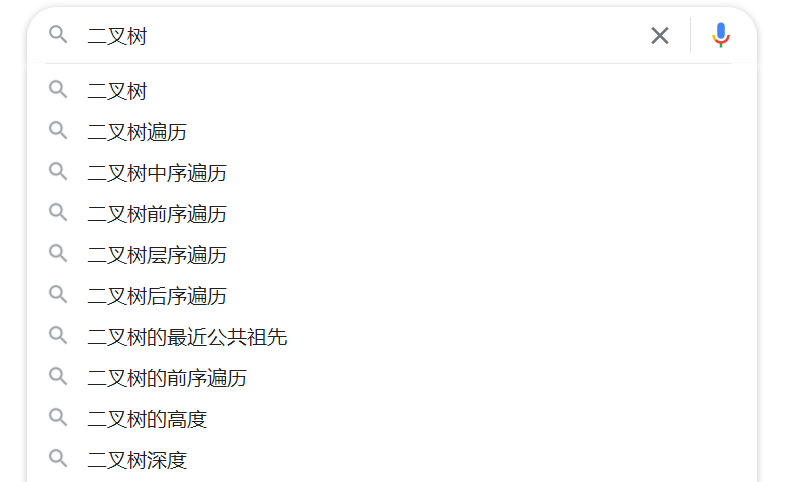
\includegraphics[scale=0.8]{img/C17/17-4/1.png}
	\caption{前缀匹配}
\end{figure}

\vspace{0.5cm}

\subsection{插入与删除}

Trie树的插入操作就是将字符串的每个字符逐一插入,插入前先判断字符对应结点是否存在,存在则共享结点,不存在则创建新结点。当字符串插入Trie树后,将该字符串最后一个字符所对应的结点中设置标志位,表示该字符为该路径上某一字符串的末尾。\\

Trie树的删除操作分为3种情况:

\begin{enumerate}
	\item 删除整个字符串:例如删除cat,从树根依次找到结点c、a、t。因为结点t为标志位,所以去除其标志位。同时结点t是叶子结点,将其删除。删除后结点a变为叶子结点,并且结点a不是标志位,也将其删除。删除后结点c变为叶子结点,并且结点c不是标志位,也将其删除。

	\item 删除前缀字符串:例如删除no,首先查找到末尾字符结点o,因为结点o不是叶子结点,只需将其标志位去除即可。

	\item 删除分支字符串:例如删除him,方法与删除整个字符串类似,区别在于当删除到共享结点h时,由于h不是叶子结点,停止删除。
\end{enumerate}

\newpage

\section{B树}

\subsection{B树}

B-树就是B树,中间的是连字符而不是减号,谁要是把B-树读成“B减树”,那可就丢人现眼了。\\

B树主要应用于文件系统以及部分数据库索引,比如著名的非关系型数据库MongoDB。数据库索引使用树型结构的原因在于树的查询效率高,而且可以保持有序。既然这样,为什么索引没有采用二叉查找树来实现呢?二叉查找树查询的时间复杂度是$ O(logn) $,性能已经足够高了,难道B树可以比它更快?\\

其实从算法逻辑上来讲,二叉查找树的查找速度和比较次数都是最小的。但是,我们不得不考虑一个现实的问题——磁盘I/O。数据库索引是存储在磁盘上的,当数据量比较大的时候,索引的大小可能有好几个G甚至更多。当利用索引查询的时候,显然不可能把整个索引全部加载到内存,能做的只有逐一加载每一页的磁盘页,这里的磁盘页就对应着索引树的结点。\\

如果利用二叉查找树作为索引结构,假设需要查询数据10,一共需要进行4次磁盘I/O。

\begin{figure}[H]
	\centering
	\begin{tikzpicture}[
			level distance=1.5cm,
			level 1/.style={sibling distance=8cm},
			level 2/.style={sibling distance=4cm},
			level 3/.style={sibling distance=2cm}
		]
		\node[circle,draw] {9}
		child {
				node[circle,draw] {5}
				child {
						node[circle,draw] {2}
						child {node[circle,draw] {1}}
						child {node[circle,draw] {3}}
					}
				child {
						node[circle,draw] {7}
						child {node[circle,draw] {6}}
						child {node[circle,draw] {8}}
					}
			}
		child {
				node[circle,draw] {13}
				child {
						node[circle,draw] {11}
						child {node[circle,draw] {10}}
						child {node[circle,draw] {12}}
					}
				child {node[circle,draw] {15}}
			};
	\end{tikzpicture}
	\caption{索引树}
\end{figure}

最坏情况下,磁盘I/O的次数等于索引树的高度。既然如此,为了减少磁盘I/O次数,就需要把原本瘦高的树结构变得矮胖,这就是B树的特征之一。\\

B树是一种多路平衡查找树,它的每一个结点最多包含k个孩子,k被称为B树的阶,k的大小取决于磁盘页的大小。\\

一个m阶的B树具有以下特征:

\begin{enumerate}
	\item 根结点至少有2个孩子。

	\item 每个中间结点都包含k - 1个元素和k个孩子($ {m \over 2} \le k \le m $)。

	\item 每个叶子结点都包含k - 1个元素($ {m \over 2} \le k \le m $)。

	\item 所有叶子结点都位于同一层。

	\item 每个结点中的元素从小到大排列,结点中k - 1个元素正好是k个孩子包含的元素的值域分划。
\end{enumerate}

例如对于一个3阶B树:

\begin{figure}[H]
	\centering
	\begin{tikzpicture}
		\tikzstyle{bplus}=[rectangle split, rectangle split horizontal,rectangle split ignore empty parts,draw, fill=white]
		\tikzstyle{every node}=[bplus]
		\tikzstyle{level 1}=[sibling distance=6cm]
		\tikzstyle{level 2}=[sibling distance=2cm]

		\node {9} [-]
		child {node {2 \nodepart{two} 6}
				child {node {1}}
				child {node {3 \nodepart{two} 5}}
				child {node {8}}
			}
		child {node {12}
				child[sibling distance=20mm] {node {11}}
				child {node {13 \nodepart{two} 15}}
			};
	\end{tikzpicture}
	\caption{3阶B树}
\end{figure}

其中结点(2, 6)包含两个元素,并且有三个孩子1、(3, 5)和8,其中1小于元素2,(3, 5)在元素2和6之间,8大于6。\\

\subsection{查询结点}

这树长得真奇怪,它真的能实现高效查询吗?\\

例如查询数据5,只需进行3次磁盘I/O。B树在查询中的比较次数其实不比二叉查找树少,尤其当单一结点中的元素数量很多时。可是相比磁盘I/O的速度,内存中的比较耗时是几乎可以忽略的。所以只要树的高度足够低,I/O次数足够少,就可以提升查询效率。相比之下结点内部元素多一些也没有关系,仅仅是多了几次内存交互,只要不超过磁盘页的大小即可。这些就是B树的优势之一。\\

\subsection{插入结点}

例如在3阶B树中插入元素4,由于结点(3, 5)已经是两元素结点,无法再增加。父结点(2, 6)也是两元素结点,也无法再增加。根结点9是单元素结点,可以升级为两元素结点。于是拆分结点(3, 5)和结点(2, 6),让根结点9升级为(4, 9),结点6独立为根结点的第二个孩子。

\begin{figure}[H]
	\centering
	\begin{tikzpicture}
		\tikzstyle{bplus}=[rectangle split, rectangle split horizontal,rectangle split ignore empty parts,draw, fill=white]
		\tikzstyle{every node}=[bplus]
		\tikzstyle{level 1}=[sibling distance=5cm]
		\tikzstyle{level 2}=[sibling distance=2cm]

		\node {4 \nodepart{two} 9} [-]
		child {node {2}
				child {node {1}}
				child {node {3}}
			}
		child {node {6}
				child {node {5}}
				child {node {8}}
			}
		child {node {12}
				child[sibling distance=20mm] {node {11}}
				child {node {13 \nodepart{two} 15}}
			};
	\end{tikzpicture}
	\caption{插入结点4}
\end{figure}

为了插入一个元素,让整个B树的那么多结点都发生了连锁改变,确实有点麻烦。但也正因为如此,让B树能够始终维持多路平衡。因此自平衡是B树的另一大优势。\\

\subsection{删除结点}

例如在3阶B树中删除元素11,删除结点11后,结点12只有一个孩子,不符合B树特征。因此找出12、13和15中的中位数13,取代结点12,而结点12下移成为第一个孩子。

\begin{figure}[H]
	\centering
	\begin{tikzpicture}
		\tikzstyle{bplus}=[rectangle split, rectangle split horizontal,rectangle split ignore empty parts,draw, fill=white]
		\tikzstyle{every node}=[bplus]
		\tikzstyle{level 1}=[sibling distance=5cm]
		\tikzstyle{level 2}=[sibling distance=2cm]

		\node {4 \nodepart{two} 9} [-]
		child {node {2}
				child {node {1}}
				child {node {3}}
			}
		child {node {6}
				child {node {5}}
				child {node {8}}
			}
		child {node {13}
				child[sibling distance=20mm] {node {12}}
				child {node {15}}
			};
	\end{tikzpicture}
	\caption{删除结点11}
\end{figure}

\newpage

\section{B+树}

\subsection{B+树}

B+树是B树的一种变体,有着比B树更高的查询性能。B+树和B树有一些共同点,但是B+树也具备一些新的特征。\\

一个m阶的B+树具有以下特征:

\begin{enumerate}
	\item 有k个子树的中间结点包含k个元素(B树中是k - 1个元素)。

	\item 所有的叶子结点中包含了全部元素的信息,及指向含这些元素记录的指针,且叶子结点本身按照关键字大小连接。

	\item 所有中间结点元素都同时存在于子结点,在子结点元素中是最大(或最小)元素。
\end{enumerate}

\begin{figure}[H]
	\centering
	\begin{tikzpicture}
		\tikzstyle{bplus}=[rectangle split, rectangle split horizontal,rectangle split ignore empty parts,draw, fill=white]
		\tikzstyle{every node}=[bplus]
		\tikzstyle{level 1}=[sibling distance=6cm]
		\tikzstyle{level 2}=[sibling distance=2cm]

		\node {8 \nodepart{two} 15} [-]
		child {node {2 \nodepart{two} 5 \nodepart{three} 8}
				child {node {1 \nodepart{two} 2}}
				child {node {3 \nodepart{two} 5}}
				child {node {6 \nodepart{two} 8}}
			}
		child {node {11 \nodepart{two} 15}
				child {node {9 \nodepart{two} 11}}
				child {node {13 \nodepart{two} 15}}
			};

		\draw[->] (-4.5,-3) -- (-3.5,-3);
		\draw[->] (-2.5,-3) -- (-1.5,-3);
		\draw[->] (-0.5,-3) -- (1.4,-3);
		\draw[->] (2.6,-3) -- (3.3,-3);
	\end{tikzpicture}
	\caption{B+树}
\end{figure}

这又是什么怪树?不但结点之间含有重复元素,而且叶子结点之间还用指针连在一起。\\

这些正是B+树的几个特性。首先,每一个父结点的元素都出现在子结点中,是子结点的最大(或最小)元素。因此根结点的最大元素也就是整个B+树的最大元素,之后无论插入或删除多少元素,始终要保持最大元素在根结点中。至于叶子结点,由于父结点的元素都出现在子结点,因此所有叶子结点包含了全部元素信息。并且每一个叶子结点都带有指向下一个结点的指针,形成了一个有序链表。\\

\subsection{单行查询}

B+树的好处主要体现在查询性能上。在单元素查询的时候,B+树会自顶向下逐层查找结点,最终找到匹配的叶子结点。例如在B+树中查询元素3,需要进行3次磁盘I/O。\\

虽然流程看起来和B树差不多,但是有两点不同。首先,B+树的中间结点并不关联数据,仅仅是索引,所以同样大小的磁盘页可以容纳更多的结点元素。这就意味着,数据量相同的情况下,B+树的结构比B树更加矮胖,因此查询时I/O次数也更少。\\

其次,B+树的查询性能必须最终查找到叶子结点,而B树只要找到匹配元素即可。因此,B树的查询性能并不稳定,最好情况下只查询根结点,最坏情况下是查到叶子结点,而B+树的每一次查询都是稳定的。\\

\subsection{范围查询}

B树中进行范围查询只能通过繁琐的中序遍历。例如在B树中查询范围为3到11的元素:

\begin{figure}[H]
	\centering
	\begin{tikzpicture}
		\tikzstyle{bplus}=[rectangle split, rectangle split horizontal,rectangle split ignore empty parts,draw, fill=white]
		\tikzstyle{every node}=[bplus]
		\tikzstyle{level 1}=[sibling distance=6cm]
		\tikzstyle{level 2}=[sibling distance=2cm]

		\node {9} [-]
		child {node {2 \nodepart{two} 6}
				child {node {1}}
				child {node {\textcolor{red}{3} \nodepart{two} \textcolor{red}{5}}}
				child {node {8}}
			}
		child {node {12}
				child[sibling distance=20mm] {node {11}}
				child {node {13 \nodepart{two} 15}}
			};
	\end{tikzpicture}
\end{figure}

\begin{figure}[H]
	\centering
	\begin{tikzpicture}
		\tikzstyle{bplus}=[rectangle split, rectangle split horizontal,rectangle split ignore empty parts,draw, fill=white]
		\tikzstyle{every node}=[bplus]
		\tikzstyle{level 1}=[sibling distance=6cm]
		\tikzstyle{level 2}=[sibling distance=2cm]

		\node {9} [-]
		child {node {2 \nodepart{two} \textcolor{red}{6}}
				child {node {1}}
				child {node {\textcolor{red}{3} \nodepart{two} \textcolor{red}{5}}}
				child {node {8}}
			}
		child {node {12}
				child[sibling distance=20mm] {node {11}}
				child {node {13 \nodepart{two} 15}}
			};
	\end{tikzpicture}
\end{figure}

\begin{figure}[H]
	\centering
	\begin{tikzpicture}
		\tikzstyle{bplus}=[rectangle split, rectangle split horizontal,rectangle split ignore empty parts,draw, fill=white]
		\tikzstyle{every node}=[bplus]
		\tikzstyle{level 1}=[sibling distance=6cm]
		\tikzstyle{level 2}=[sibling distance=2cm]

		\node {9} [-]
		child {node {2 \nodepart{two} \textcolor{red}{6}}
				child {node {1}}
				child {node {\textcolor{red}{3} \nodepart{two} \textcolor{red}{5}}}
				child {node {\textcolor{red}{8}}}
			}
		child {node {12}
				child[sibling distance=20mm] {node {11}}
				child {node {13 \nodepart{two} 15}}
			};
	\end{tikzpicture}
\end{figure}

\begin{figure}[H]
	\centering
	\begin{tikzpicture}
		\tikzstyle{bplus}=[rectangle split, rectangle split horizontal,rectangle split ignore empty parts,draw, fill=white]
		\tikzstyle{every node}=[bplus]
		\tikzstyle{level 1}=[sibling distance=6cm]
		\tikzstyle{level 2}=[sibling distance=2cm]

		\node {\textcolor{red}{9}} [-]
		child {node {2 \nodepart{two} \textcolor{red}{6}}
				child {node {1}}
				child {node {\textcolor{red}{3} \nodepart{two} \textcolor{red}{5}}}
				child {node {\textcolor{red}{8}}}
			}
		child {node {12}
				child[sibling distance=20mm] {node {11}}
				child {node {13 \nodepart{two} 15}}
			};
	\end{tikzpicture}
\end{figure}

\begin{figure}[H]
	\centering
	\begin{tikzpicture}
		\tikzstyle{bplus}=[rectangle split, rectangle split horizontal,rectangle split ignore empty parts,draw, fill=white]
		\tikzstyle{every node}=[bplus]
		\tikzstyle{level 1}=[sibling distance=6cm]
		\tikzstyle{level 2}=[sibling distance=2cm]

		\node {\textcolor{red}{9}} [-]
		child {node {2 \nodepart{two} \textcolor{red}{6}}
				child {node {1}}
				child {node {\textcolor{red}{3} \nodepart{two} \textcolor{red}{5}}}
				child {node {\textcolor{red}{8}}}
			}
		child {node {12}
				child[sibling distance=20mm] {node {\textcolor{red}{11}}}
				child {node {13 \nodepart{two} 15}}
			};
	\end{tikzpicture}
\end{figure}

反观B+树的范围查询,则要简单的多,只需要在链表上做遍历即可:\\

\begin{figure}[H]
	\centering
	\begin{tikzpicture}
		\tikzstyle{bplus}=[rectangle split, rectangle split horizontal,rectangle split ignore empty parts,draw, fill=white]
		\tikzstyle{every node}=[bplus]
		\tikzstyle{level 1}=[sibling distance=6cm]
		\tikzstyle{level 2}=[sibling distance=2cm]

		\node {8 \nodepart{two} 15} [-]
		child {node {2 \nodepart{two} 5 \nodepart{three} 8}
				child {node {1 \nodepart{two} 2}}
				child {node {\textcolor{red}{3} \nodepart{two} \textcolor{red}{5}}}
				child {node {6 \nodepart{two} 8}}
			}
		child {node {11 \nodepart{two} 15}
				child {node {9 \nodepart{two} 11}}
				child {node {13 \nodepart{two} 15}}
			};

		\draw[->] (-4.5,-3) -- (-3.5,-3);
		\draw[->] (-2.5,-3) -- (-1.5,-3);
		\draw[->] (-0.5,-3) -- (1.4,-3);
		\draw[->] (2.6,-3) -- (3.3,-3);
	\end{tikzpicture}
\end{figure}

\begin{figure}[H]
	\centering
	\begin{tikzpicture}
		\tikzstyle{bplus}=[rectangle split, rectangle split horizontal,rectangle split ignore empty parts,draw, fill=white]
		\tikzstyle{every node}=[bplus]
		\tikzstyle{level 1}=[sibling distance=6cm]
		\tikzstyle{level 2}=[sibling distance=2cm]

		\node {8 \nodepart{two} 15} [-]
		child {node {2 \nodepart{two} 5 \nodepart{three} 8}
				child {node {1 \nodepart{two} 2}}
				child {node {\textcolor{red}{3} \nodepart{two} \textcolor{red}{5}}}
				child {node {\textcolor{red}{6} \nodepart{two} \textcolor{red}{8}}}
			}
		child {node {11 \nodepart{two} 15}
				child {node {9 \nodepart{two} 11}}
				child {node {13 \nodepart{two} 15}}
			};

		\draw[->] (-4.5,-3) -- (-3.5,-3);
		\draw[->] (-2.5,-3) -- (-1.5,-3);
		\draw[->] (-0.5,-3) -- (1.4,-3);
		\draw[->] (2.6,-3) -- (3.3,-3);
	\end{tikzpicture}
\end{figure}

\begin{figure}[H]
	\centering
	\begin{tikzpicture}
		\tikzstyle{bplus}=[rectangle split, rectangle split horizontal,rectangle split ignore empty parts,draw, fill=white]
		\tikzstyle{every node}=[bplus]
		\tikzstyle{level 1}=[sibling distance=6cm]
		\tikzstyle{level 2}=[sibling distance=2cm]

		\node {8 \nodepart{two} 15} [-]
		child {node {2 \nodepart{two} 5 \nodepart{three} 8}
				child {node {1 \nodepart{two} 2}}
				child {node {\textcolor{red}{3} \nodepart{two} \textcolor{red}{5}}}
				child {node {\textcolor{red}{6} \nodepart{two} \textcolor{red}{8}}}
			}
		child {node {11 \nodepart{two} 15}
				child {node {\textcolor{red}{9} \nodepart{two} \textcolor{red}{11}}}
				child {node {13 \nodepart{two} 15}}
			};

		\draw[->] (-4.5,-3) -- (-3.5,-3);
		\draw[->] (-2.5,-3) -- (-1.5,-3);
		\draw[->] (-0.5,-3) -- (1.4,-3);
		\draw[->] (2.6,-3) -- (3.3,-3);
	\end{tikzpicture}
\end{figure}

\newpage

\section{并查集}

\subsection{并查集(Disjoint Set)}

并查集是一种简洁优雅的数据结构,主要用于解决一些元素分组的问题。\\

它管理一系列不相交的集合,并支持两种操作:

\begin{enumerate}
	\item 合并(union):把两个不相交的集合合并为一个集合。
	\item 查询(find):查询两个元素是否在同一个集合中。
\end{enumerate}

例如在某个家族中,如果x和y是亲戚,y和z是亲戚,那么x和z也是亲戚。如果x和y是亲戚,那么x的亲戚都是y的亲戚,y的亲戚也都是x的亲戚。为了判断两个人是否为亲戚,只需判断他们是否属于同一个集合即可。\\

并查集的思想在于用集合中的一个元素代表集合,类似于把集合看做帮派,代表元素则是帮主,最开始所有元素各自为一个集合(各自的帮主就是自己)。

\begin{figure}[H]
	\centering
	\begin{tikzpicture}
		\node[circle,minimum width=30pt,minimum height=30pt,draw=black] (1) at(0,0){1};
		\node[circle,minimum width=30pt,minimum height=30pt,draw=black] (2) at(2,2){2};
		\node[circle,minimum width=30pt,minimum height=30pt,draw=black] (3) at(4,-2){3};
		\node[circle,minimum width=30pt,minimum height=30pt,draw=black] (4) at(6,0){4};
		\node[circle,minimum width=30pt,minimum height=30pt,draw=black] (5) at(8,-2){5};
		\node[circle,minimum width=30pt,minimum height=30pt,draw=black] (6) at(10,2){6};

		\draw[->] (1) to[out=90,in=180,loop,looseness=4.8] (1);
		\draw[->] (2) to[out=90,in=180,loop,looseness=4.8] (2);
		\draw[->] (3) to[out=90,in=180,loop,looseness=4.8] (3);
		\draw[->] (4) to[out=90,in=180,loop,looseness=4.8] (4);
		\draw[->] (5) to[out=90,in=180,loop,looseness=4.8] (5);
		\draw[->] (6) to[out=90,in=180,loop,looseness=4.8] (6);
	\end{tikzpicture}
\end{figure}

例如将元素1和3合并,就是将1和3比武,假设1赢了,3就认1作帮主。

\begin{figure}[H]
	\centering
	\begin{tikzpicture}
		\node[circle,minimum width=30pt,minimum height=30pt,draw=black] (1) at(0,0){1};
		\node[circle,minimum width=30pt,minimum height=30pt,draw=black] (2) at(2,2){2};
		\node[circle,minimum width=30pt,minimum height=30pt,draw=black] (3) at(4,-2){3};
		\node[circle,minimum width=30pt,minimum height=30pt,draw=black] (4) at(6,0){4};
		\node[circle,minimum width=30pt,minimum height=30pt,draw=black] (5) at(8,-2){5};
		\node[circle,minimum width=30pt,minimum height=30pt,draw=black] (6) at(10,2){6};

		\draw[->] (1) to[out=90,in=180,loop,looseness=4.8] (1);
		\draw[->] (2) to[out=90,in=180,loop,looseness=4.8] (2);
		\draw[->] (3) to[bend left] (1);
		\draw[->] (4) to[out=90,in=180,loop,looseness=4.8] (4);
		\draw[->] (5) to[out=90,in=180,loop,looseness=4.8] (5);
		\draw[->] (6) to[out=90,in=180,loop,looseness=4.8] (6);
	\end{tikzpicture}
	\caption{合并1和3}
\end{figure}

再合并元素2和3,但3表示“别跟我打,让我的帮主来收拾你”。假设还是1赢了,2也认1作帮主。

\begin{figure}[H]
	\centering
	\begin{tikzpicture}
		\node[circle,minimum width=30pt,minimum height=30pt,draw=black] (1) at(0,0){1};
		\node[circle,minimum width=30pt,minimum height=30pt,draw=black] (2) at(2,2){2};
		\node[circle,minimum width=30pt,minimum height=30pt,draw=black] (3) at(4,-2){3};
		\node[circle,minimum width=30pt,minimum height=30pt,draw=black] (4) at(6,0){4};
		\node[circle,minimum width=30pt,minimum height=30pt,draw=black] (5) at(8,-2){5};
		\node[circle,minimum width=30pt,minimum height=30pt,draw=black] (6) at(10,2){6};

		\draw[->] (1) to[out=90,in=180,loop,looseness=4.8] (1);
		\draw[->] (2) to[bend right] (1);
		\draw[->] (3) to[bend left] (1);
		\draw[->] (4) to[out=90,in=180,loop,looseness=4.8] (4);
		\draw[->] (5) to[out=90,in=180,loop,looseness=4.8] (5);
		\draw[->] (6) to[out=90,in=180,loop,looseness=4.8] (6);
	\end{tikzpicture}
	\caption{合并2和3}
\end{figure}

假设元素4、5、6也进行了相关合并:

\begin{figure}[H]
	\centering
	\begin{tikzpicture}
		\node[circle,minimum width=30pt,minimum height=30pt,draw=black] (1) at(0,0){1};
		\node[circle,minimum width=30pt,minimum height=30pt,draw=black] (2) at(2,2){2};
		\node[circle,minimum width=30pt,minimum height=30pt,draw=black] (3) at(4,-2){3};
		\node[circle,minimum width=30pt,minimum height=30pt,draw=black] (4) at(6,0){4};
		\node[circle,minimum width=30pt,minimum height=30pt,draw=black] (5) at(8,-2){5};
		\node[circle,minimum width=30pt,minimum height=30pt,draw=black] (6) at(10,2){6};

		\draw[->] (1) to[out=90,in=180,loop,looseness=4.8] (1);
		\draw[->] (2) to[bend right] (1);
		\draw[->] (3) to[bend left] (1);
		\draw[->] (4) to[out=90,in=180,loop,looseness=4.8] (4);
		\draw[->] (5) to[bend left] (4);
		\draw[->] (6) to[bend right] (4);
	\end{tikzpicture}
	\caption{合并4、5、6}
\end{figure}

现在再合并元素2和6,将它们的帮主1和4比武,假设1胜利后,4认1为帮主,当然它的手下也都跟着投降了。

\begin{figure}[H]
	\centering
	\begin{tikzpicture}
		\node[circle,minimum width=30pt,minimum height=30pt,draw=black] (1) at(0,0){1};
		\node[circle,minimum width=30pt,minimum height=30pt,draw=black] (2) at(2,2){2};
		\node[circle,minimum width=30pt,minimum height=30pt,draw=black] (3) at(4,-2){3};
		\node[circle,minimum width=30pt,minimum height=30pt,draw=black] (4) at(6,0){4};
		\node[circle,minimum width=30pt,minimum height=30pt,draw=black] (5) at(8,-2){5};
		\node[circle,minimum width=30pt,minimum height=30pt,draw=black] (6) at(10,2){6};

		\draw[->] (1) to[out=90,in=180,loop,looseness=4.8] (1);
		\draw[->] (2) to[bend right] (1);
		\draw[->] (3) to[bend left] (1);
		\draw[->] (4) -- (1);
		\draw[->] (5) to[bend left] (4);
		\draw[->] (6) to[bend right] (4);
	\end{tikzpicture}
	\caption{合并2和6}
\end{figure}

并查集是一种树型结构,要寻找集合的代表元素,只需要一层一层向上访问父结点,直达树的根结点即可。根结点的父结点就是它自己。\\

假设有n个元素,利用数组parent存放每个元素的父结点,一开始每个元素的父结点为自己。\\

\mybox{初始化}

\begin{lstlisting}[language=C]
void init(int n) {
    parent = (int *)malloc(sizeof(int) * n);
    for(int i = 0; i < n; i++) {
        parent[i] = i;
    }
}
\end{lstlisting}

要判断两个元素是否属于同一个集合,只需要看它们的根结点是否相同。利用递归的方法可以实现对代表元素的查询,一层一层访问父结点,直至根结点。\\

\mybox{查询}

\begin{lstlisting}[language=C]
int find(int val) {
    if(parent[val] == val) {
        return val;
    }
    return find(parent[val]);
}
\end{lstlisting}

合并操作需要先找到两个集合的根结点,将前者的父结点设置为后者即可(也可将后者的父结点设置为前者)。\\

\mybox{合并}

\begin{lstlisting}[language=C]
void merge(int i, int j) {
    parent[find(i)] = find(j);
}
\end{lstlisting}

\vspace{0.5cm}

\subsection{路径压缩(Path Compression)}

最简单的并查集效率是比较低的,分别进行merge(2, 3)和merge(2, 4):

\begin{figure}[H]
	\centering
	\begin{tikzpicture}
		\node[circle,minimum width=30pt,minimum height=30pt,draw=black] (1) at(0,0){1};
		\node[circle,minimum width=30pt,minimum height=30pt,draw=black] (2) at(0,-2){2};
		\node[circle,minimum width=30pt,minimum height=30pt,draw=black] (3) at(3,-1){3};
		\node[circle,minimum width=30pt,minimum height=30pt,draw=black] (4) at(6,-1){4};

		\draw[->] (1) to[out=370,in=115,loop,looseness=4.8] (1);
		\draw[->] (2) -- (1);
		\draw[->] (3) to[out=370,in=115,loop,looseness=4.8] (3);
		\draw[->] (4) to[out=370,in=115,loop,looseness=4.8] (4);
	\end{tikzpicture}
\end{figure}

\begin{figure}[H]
	\centering
	\begin{tikzpicture}
		\node[circle,minimum width=30pt,minimum height=30pt,draw=black] (1) at(0,0){1};
		\node[circle,minimum width=30pt,minimum height=30pt,draw=black] (2) at(0,-2){2};
		\node[circle,minimum width=30pt,minimum height=30pt,draw=black] (3) at(0,2){3};
		\node[circle,minimum width=30pt,minimum height=30pt,draw=black] (4) at(3,0){4};

		\draw[->] (1) -- (3);
		\draw[->] (2) -- (1);
		\draw[->] (3) to[out=370,in=115,loop,looseness=4.8] (3);
		\draw[->] (4) to[out=370,in=115,loop,looseness=4.8] (4);
	\end{tikzpicture}
\end{figure}

\begin{figure}[H]
	\centering
	\begin{tikzpicture}
		\node[circle,minimum width=30pt,minimum height=30pt,draw=black] (1) at(0,0){1};
		\node[circle,minimum width=30pt,minimum height=30pt,draw=black] (2) at(0,-2){2};
		\node[circle,minimum width=30pt,minimum height=30pt,draw=black] (3) at(0,2){3};
		\node[circle,minimum width=30pt,minimum height=30pt,draw=black] (4) at(0,4){4};

		\draw[->] (1) -- (3);
		\draw[->] (2) -- (1);
		\draw[->] (3) -- (4);
		\draw[->] (4) to[out=370,in=115,loop,looseness=4.8] (4);
	\end{tikzpicture}
\end{figure}

这样可能会形成一条长链,随着链越来越长,想要从底部找到根结点会变得越来越难。利用路径压缩的方法可以解决这个问题,因为我们只关心一个元素所对应的根结点,因此每个元素到根结点的路径最好尽可能短。\\

实现的时候只需在查询过程中,把沿途的每个结点的父结点都设置为根结点即可。在下一次查询的时候,就可以节省很多时间。

\begin{figure}[H]
	\centering
	\begin{tikzpicture}
		\node[circle,minimum width=30pt,minimum height=30pt,draw=black] (1) at(0,0){1};
		\node[circle,minimum width=30pt,minimum height=30pt,draw=black] (2) at(0,-2){2};
		\node[circle,minimum width=30pt,minimum height=30pt,draw=black] (3) at(0,2){3};
		\node[circle,minimum width=30pt,minimum height=30pt,draw=black] (4) at(0,4){4};

		\draw[->] (1) to[bend left] (4);
		\draw[->] (2) to[bend right] (4);
		\draw[->] (3) -- (4);
		\draw[->] (4) to[out=370,in=115,loop,looseness=4.8] (4);
	\end{tikzpicture}
\end{figure}

\mybox{查询(路径压缩)}

\begin{lstlisting}[language=C]
int find(int val) {
    if(parent[val] == val) {
        return val;
    } else {
        parent[val] = find(parent[val]);
        return parent[val];
    }
}
\end{lstlisting}

\vspace{0.5cm}

\subsection{按秩合并}

如果需要将一棵比较复杂的树与一个单元素进行合并,例如merge(7, 8)时,是把元素7的父结点设为8好,还是把8的父结点设为7呢?

\begin{figure}[H]
	\centering
	\begin{tikzpicture}
		\node[circle,minimum width=30pt,minimum height=30pt,draw=black] (1) at(0,0){1};
		\node[circle,minimum width=30pt,minimum height=30pt,draw=black] (2) at(2,0){2};
		\node[circle,minimum width=30pt,minimum height=30pt,draw=black] (3) at(4,0){3};
		\node[circle,minimum width=30pt,minimum height=30pt,draw=black] (4) at(1,2){4};
		\node[circle,minimum width=30pt,minimum height=30pt,draw=black] (5) at(3,2){5};
		\node[circle,minimum width=30pt,minimum height=30pt,draw=black] (6) at(2,4){6};
		\node[circle,minimum width=30pt,minimum height=30pt,draw=black] (7) at(2,6){7};
		\node[circle,minimum width=30pt,minimum height=30pt,draw=black] (8) at(6,3){8};

		\draw[->] (1) -- (4);
		\draw[->] (2) -- (4);
		\draw[->] (3) -- (5);
		\draw[->] (4) -- (6);
		\draw[->] (5) -- (6);
		\draw[->] (6) -- (7);
		\draw[->] (7) to[out=370,in=115,loop,looseness=4.8] (7);
		\draw[->] (8) to[out=370,in=115,loop,looseness=4.8] (8);
	\end{tikzpicture}
\end{figure}

如果把7的父结点设为8,会使树的深度加深,原来树中的每个元素到根结点的距离都变长了,之后寻找根结点的路径也会变长。虽然有路径压缩,但路径压缩也是要消耗时间的。而把8的父结点设为7,并不会影响到不相关的结点。

\begin{figure}[H]
	\centering
	\begin{tikzpicture}
		\node[circle,minimum width=30pt,minimum height=30pt,draw=black] (1) at(0,0){1};
		\node[circle,minimum width=30pt,minimum height=30pt,draw=black] (2) at(2,0){2};
		\node[circle,minimum width=30pt,minimum height=30pt,draw=black] (3) at(4,0){3};
		\node[circle,minimum width=30pt,minimum height=30pt,draw=black] (4) at(1,2){4};
		\node[circle,minimum width=30pt,minimum height=30pt,draw=black] (5) at(3,2){5};
		\node[circle,minimum width=30pt,minimum height=30pt,draw=black] (6) at(2,4){6};
		\node[circle,minimum width=30pt,minimum height=30pt,draw=black] (7) at(3,6){7};
		\node[circle,minimum width=30pt,minimum height=30pt,draw=black] (8) at(4,4){8};

		\draw[->] (1) -- (4);
		\draw[->] (2) -- (4);
		\draw[->] (3) -- (5);
		\draw[->] (4) -- (6);
		\draw[->] (5) -- (6);
		\draw[->] (6) -- (7);
		\draw[->] (7) to[out=370,in=115,loop,looseness=4.8] (7);
		\draw[->] (8) -- (7);
	\end{tikzpicture}
\end{figure}

因此在合并两个集合时,应该把简单的树往复杂的树上合并。利用数组rank记录每个结点对应的树的深度,一开始所有元素的rank设为1。合并时比较两个根结点,把rank较小者往较大者上合并。深度相同的情况下,无论如何合并,都会使树的深度增加1。\\

\mybox{按秩合并}

\begin{lstlisting}[language=C]
void init(int n) {
    parent = (int *)malloc(sizeof(int) * n);
    rank = (int *)malloc(sizeof(int) * n);
    for(int i = 0; i < n; i++) {
        parent[i] = i;
        rank[i] = 1;
    }
}

void merge(int i, int j) {
    // 找到对应根结点
    int x = find(i);
    int y = find(j);
    if(rank[x] <= rank[y]) {
        parent[x] = y;
    } else {
        parent[y] = x;
    }
    // 如果深度相同且根结点不同,则新的根结点深度+1
    if(rank[x] == rank[y] && x != y) {
        rank[y]++;
    }
}
\end{lstlisting}